In this chapter, we will look at the results we found and talk about stability analysis of the CGLE with four different
potential functions.

\section{ Generation of Cavity solitons}
First, we generate cavity solitons by numerically solving the governing CGLE following SSFM. A typical set of CS is presented in figure below Fig: \ref{fig:CS without potential}.

\begin{figure}[H]
    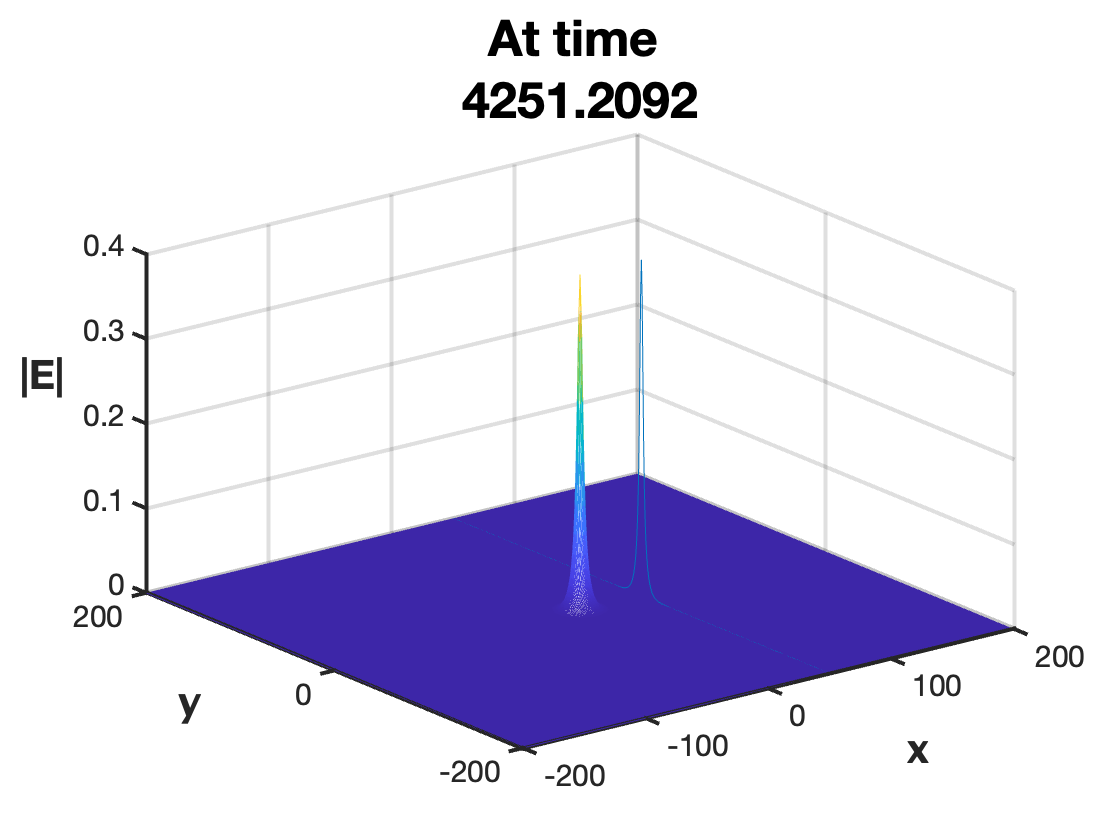
\includegraphics[scale=0.225]{CGLE without potential.png}
    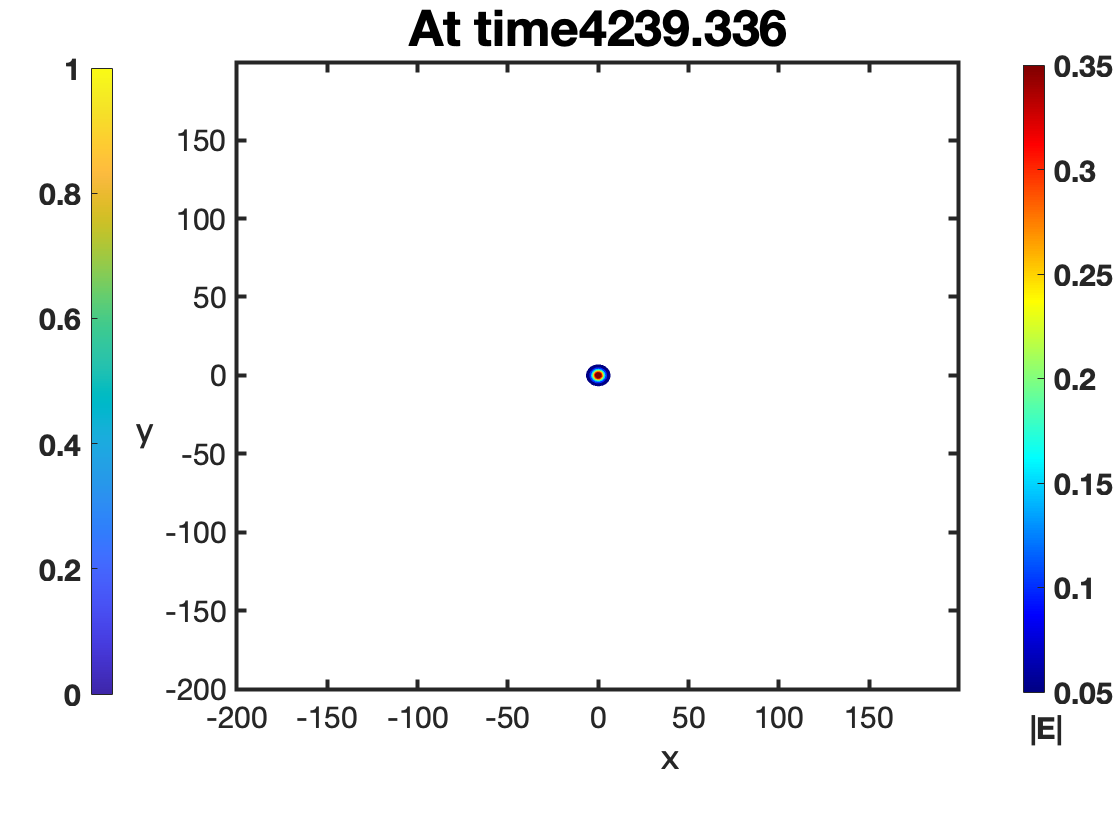
\includegraphics[scale=0.225]{CGLE without potential cont.png}
    \caption{Cavity Soliton generation without any potential}
    \label{fig:CS without potential}
\end{figure}

Now, we use a potential to trap the generated CS. Four such different potentials have been used. 
The following are the numerical simulation of CGLE with different spatially varying transverse potential\
functions, all of which have central peaks. The aim here is to trap CS near or on the\
central peak of the applied potential. This helps in effective manipulation of CS which have many\
technological applications.

\paragraph{Assumptions:} The following parameter values were initially found using analytical approximation like discussed above lagrangian variational method. 
$\theta = 1.1$, $\mu = 1.37$, $\alpha =2.7$,$\gamma =0.55$, $\beta = 1.4$,$s = 10$,\ 
$g_1=g_2=G=4$,
feedback bandwidth $\lambda = 0.6$, 
feedback strength $\sigma =0.4$, 
resonance frequency $\omega_0 = 1.2$,
Amplitude of CS $A=0.25$,
unsaturable absorption parameter $\alpha_{NS}= 0.020$.

These values are used to define our system and only on subsequent numerical simulations were altered based on the need.
Otherwise they were mostly kept constant so that overall our system is unchanged except for the change in potential which is introduced by\
us.  

We have also considered a symmetric system as far as the spatial geometry is concerned. This is a valid assumption because we generally have\
the ability to make the geometry of our instruments precise. That is exactly what has been assumed for our VCSEL system. 

\subsection{Sinc potential with Gaussian wave profile:}
In this configuration, we have CGLE with Sinc potential function. Sinc function in 2D has\
a central peak at $(0,0)$ with concentric rings of diminishing amplitude surrounding it as can be\
seen in (\ref{fig:2D_Sinc_potential}).  

\begin{figure}[h!]
    \centering
    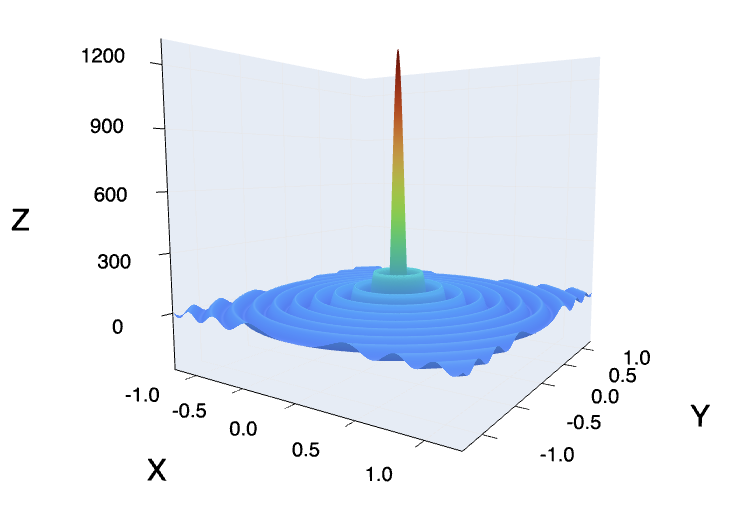
\includegraphics[scale=0.75]{sinc potential profile.png}
    \caption{Sinc function in 2D with central peak}
        \label{fig:2D_Sinc_potential}
\end{figure}

The Gaussian driving beam is used 

\begin{figure}[h!]
    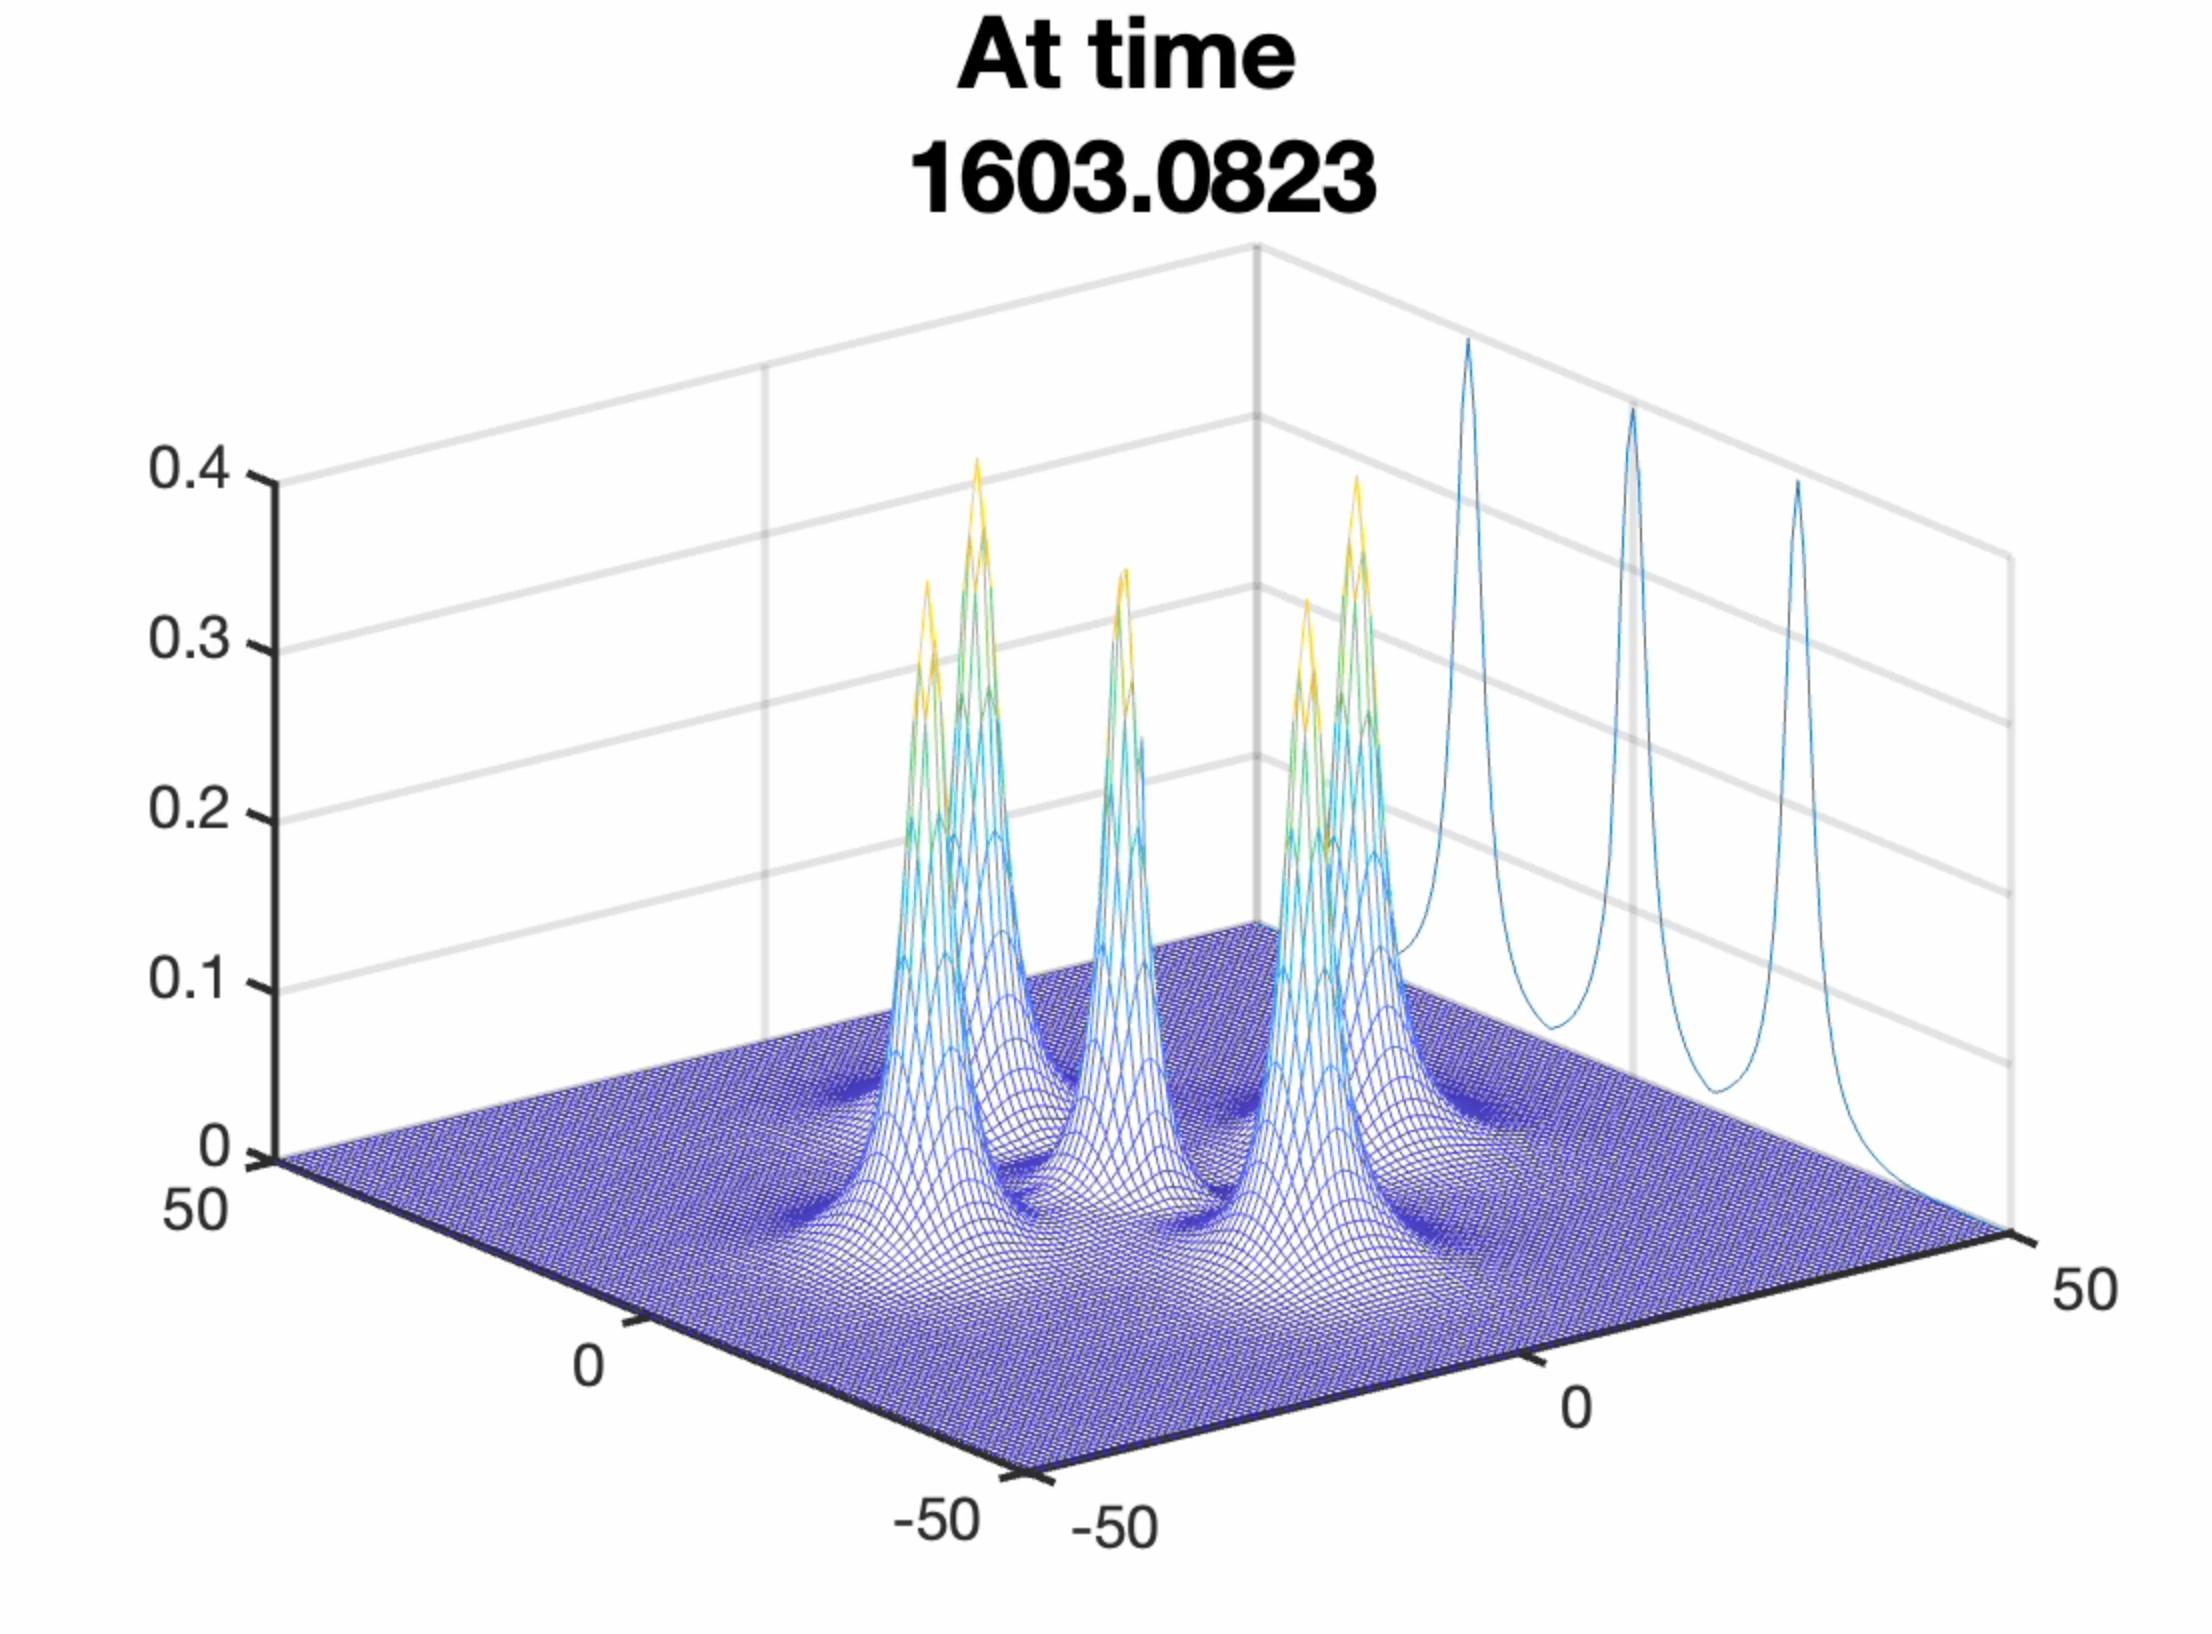
\includegraphics[scale=0.225]{44-12.998.png}
    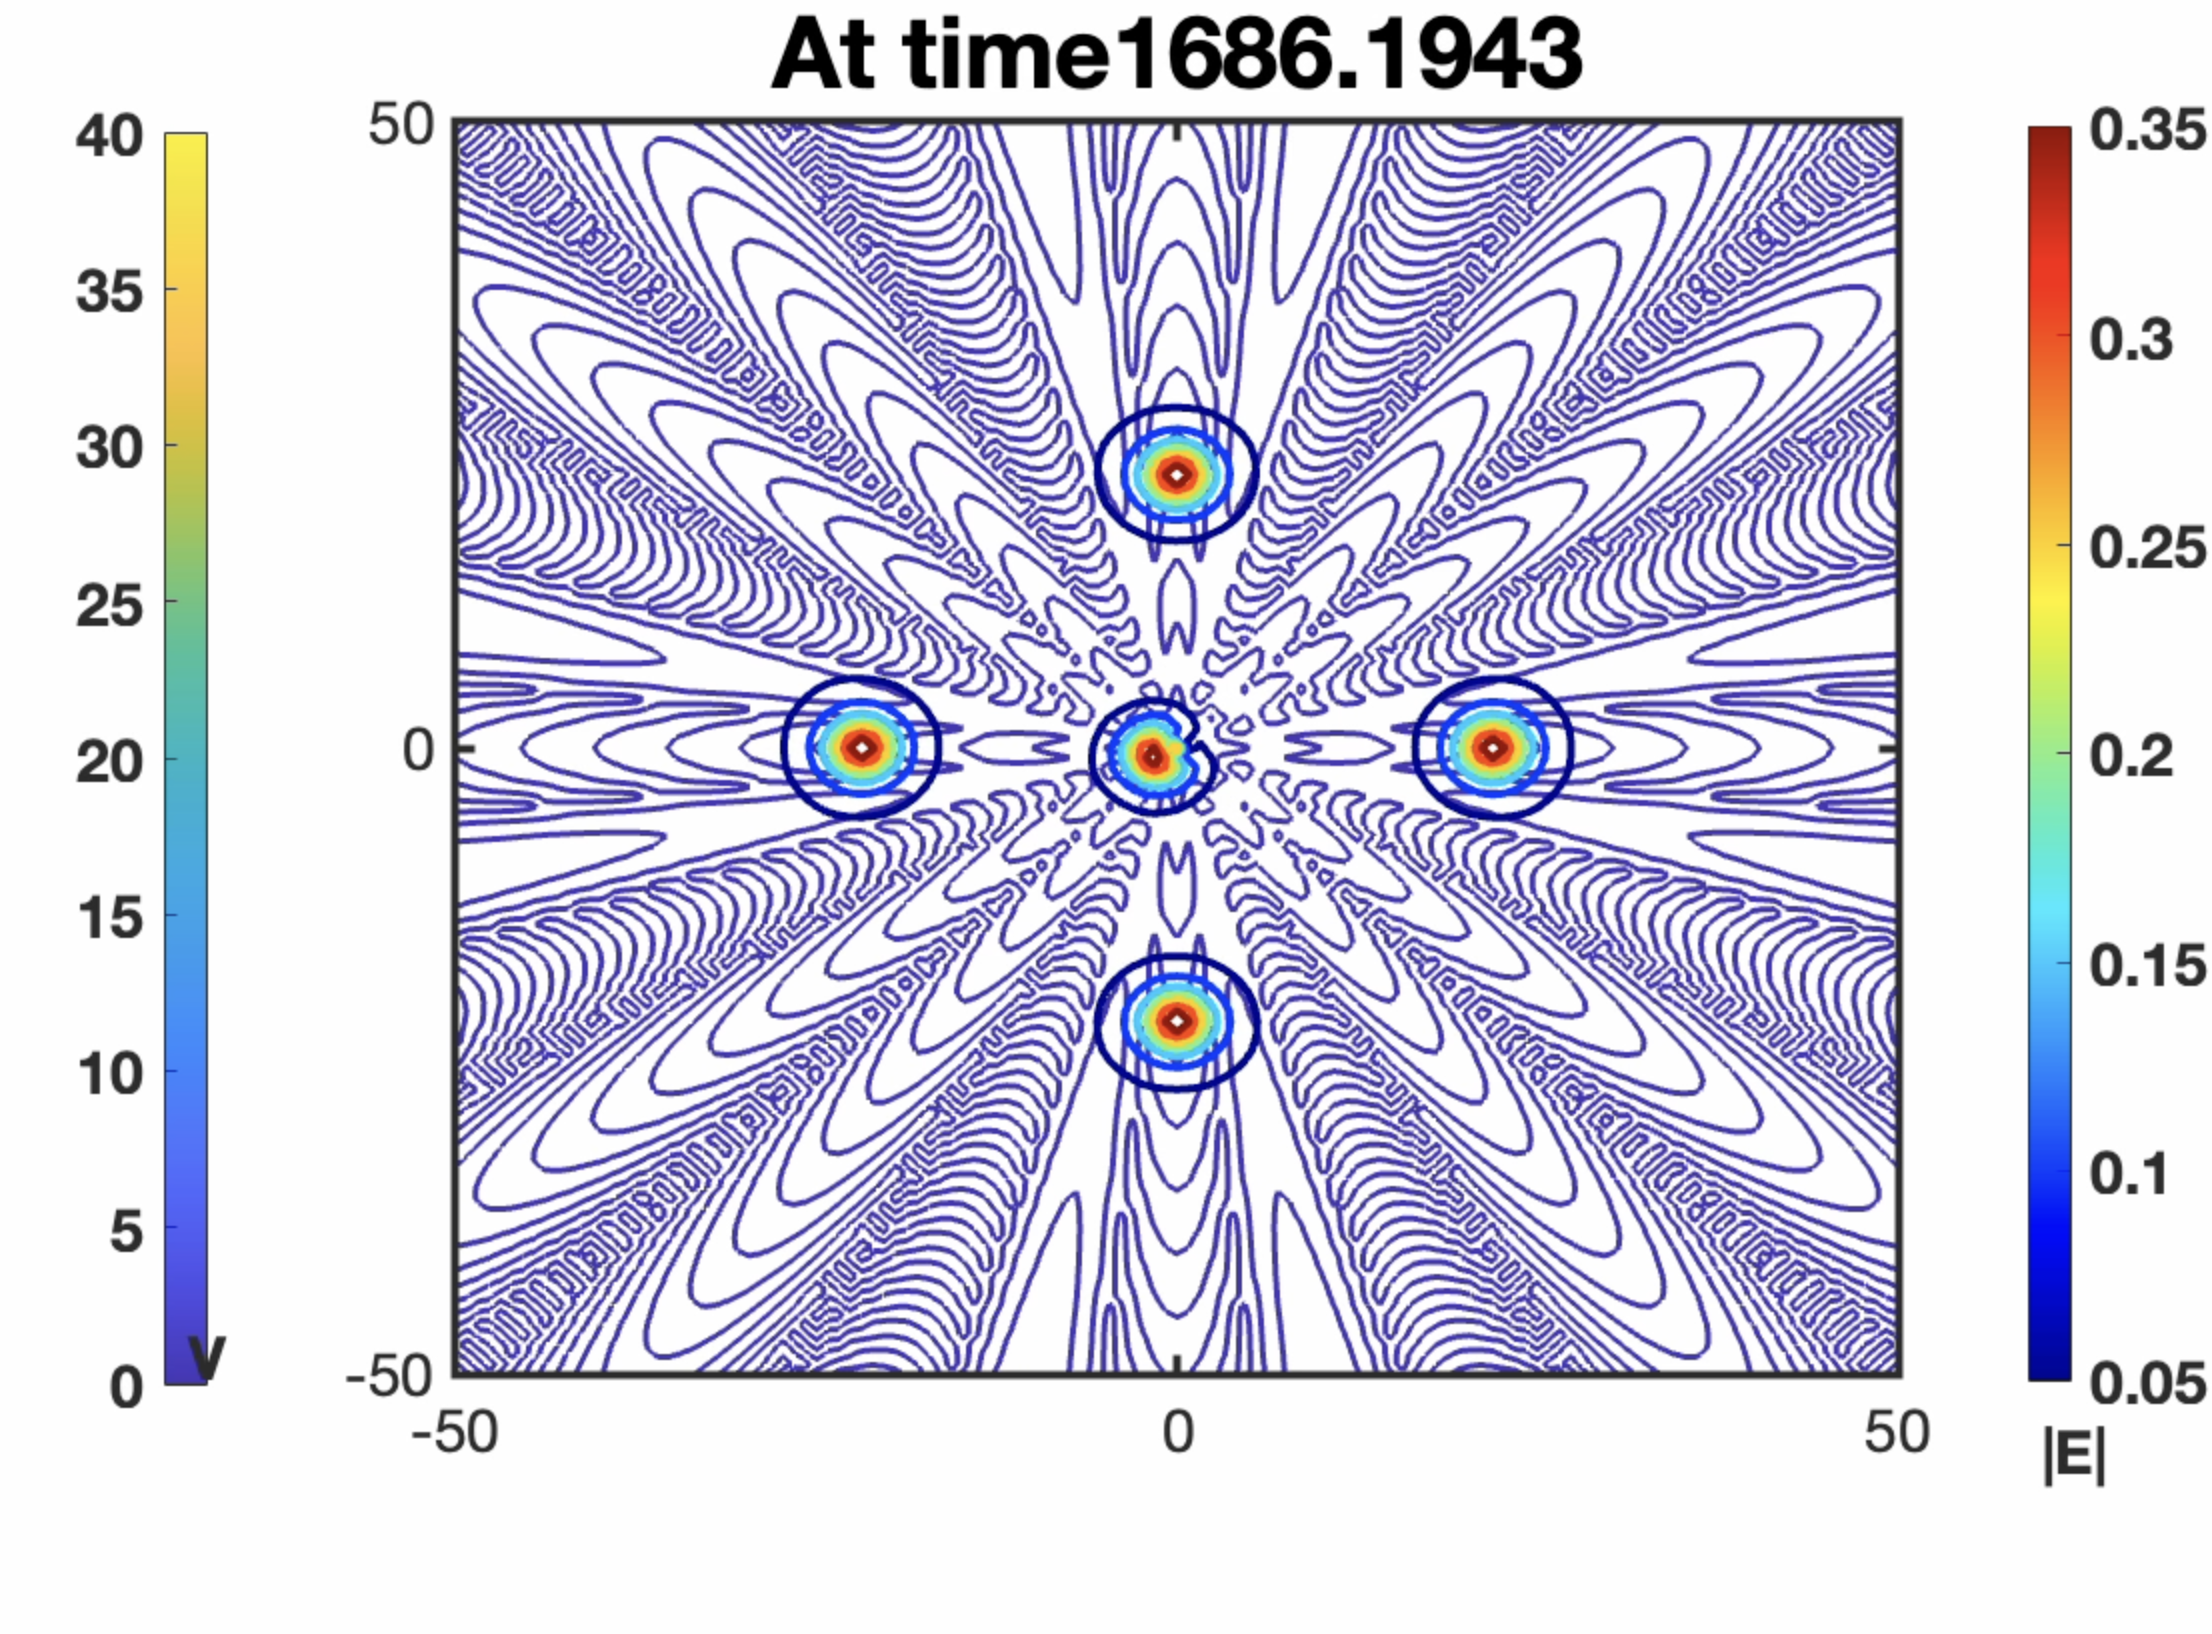
\includegraphics[scale=0.225]{44-12.998 cont.png}
    \caption{Solitons in Sinc Potential with gaussian wave profile showing five pillars}
    \label{fig:Sinc_with_gaussian_profile}
\end{figure}

\begin{enumerate}
    \item Here we have four stable peaks (CS) that maintain their position and then we have another which is trapped aroud the peak of the\ 
    potential and keeps rotating around it. 
    \item  We have also found that this system is highly sensitive to the frequence of concentric peaks\ 
    occuring in the applied potential and relatively less sensitive to the hight of the potential.
    \item For the given parameters mentioned above, the range of potential height in which the phenomenon occurs is {\bf43.300- 49.723}
    \item the range for potential frequency is {\bf 12.998-13.125}
\end{enumerate}
    

\subsection{TCMSG potential with Gaussian wave profile:}

The TCMSG profile \cite{sunPatternTransformationControl} is a compound function has two peaks and two valleys around the center as shown in fig (\ref{fig:TCMSG_profile1})
and (\ref{fig:TCMSG_profile1_ariel}) is given as:
\begin{equation}
    V(x,y) = A \sin\left(\delta\frac{xy}{\omega_0^2}\right) \exp\left(\frac{-x^2-y^2}{\omega_0^2}\right) \label{TCMSG_eqn}
\end{equation}
\begin{figure}[h!]
    \begin{subfigure}{0.5\textwidth}
        \includegraphics[scale=0.5]{TCMSG profile.png}
        \caption{}
        \label{fig:TCMSG_profile1}
    \end{subfigure}
    \begin{subfigure}{0.5\textwidth}
        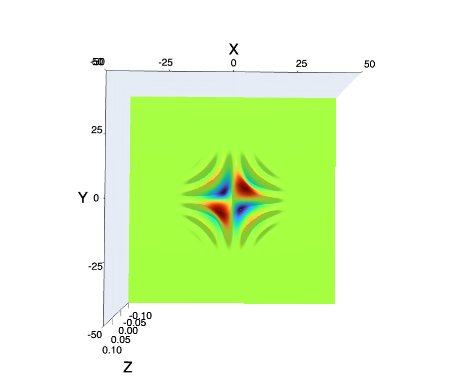
\includegraphics[scale=0.5]{TCMSG Profile(ariel view).png}
        \caption{}
        \label{fig:TCMSG_profile1_ariel}
    \end{subfigure}
    \caption{TCMSG Plots (a) shows the side view (b) shows the ariel view}
\end{figure}

For this system, with input profile being Gaussian, we see that solitons are nicely trapped around the center\
on the peaks an valleys as shown in fig (\ref{fig:TCMSG_with_gaussian_profile}). The ones which are in valleys, exhibit more stability than those that are on the peak. This is\
evident in the simulation where the solitons on the peaks can be seen to be shaking throughout the cycle and are first to\
decay upon any change in either parameters or external interference. 
\begin{figure}[h!]
        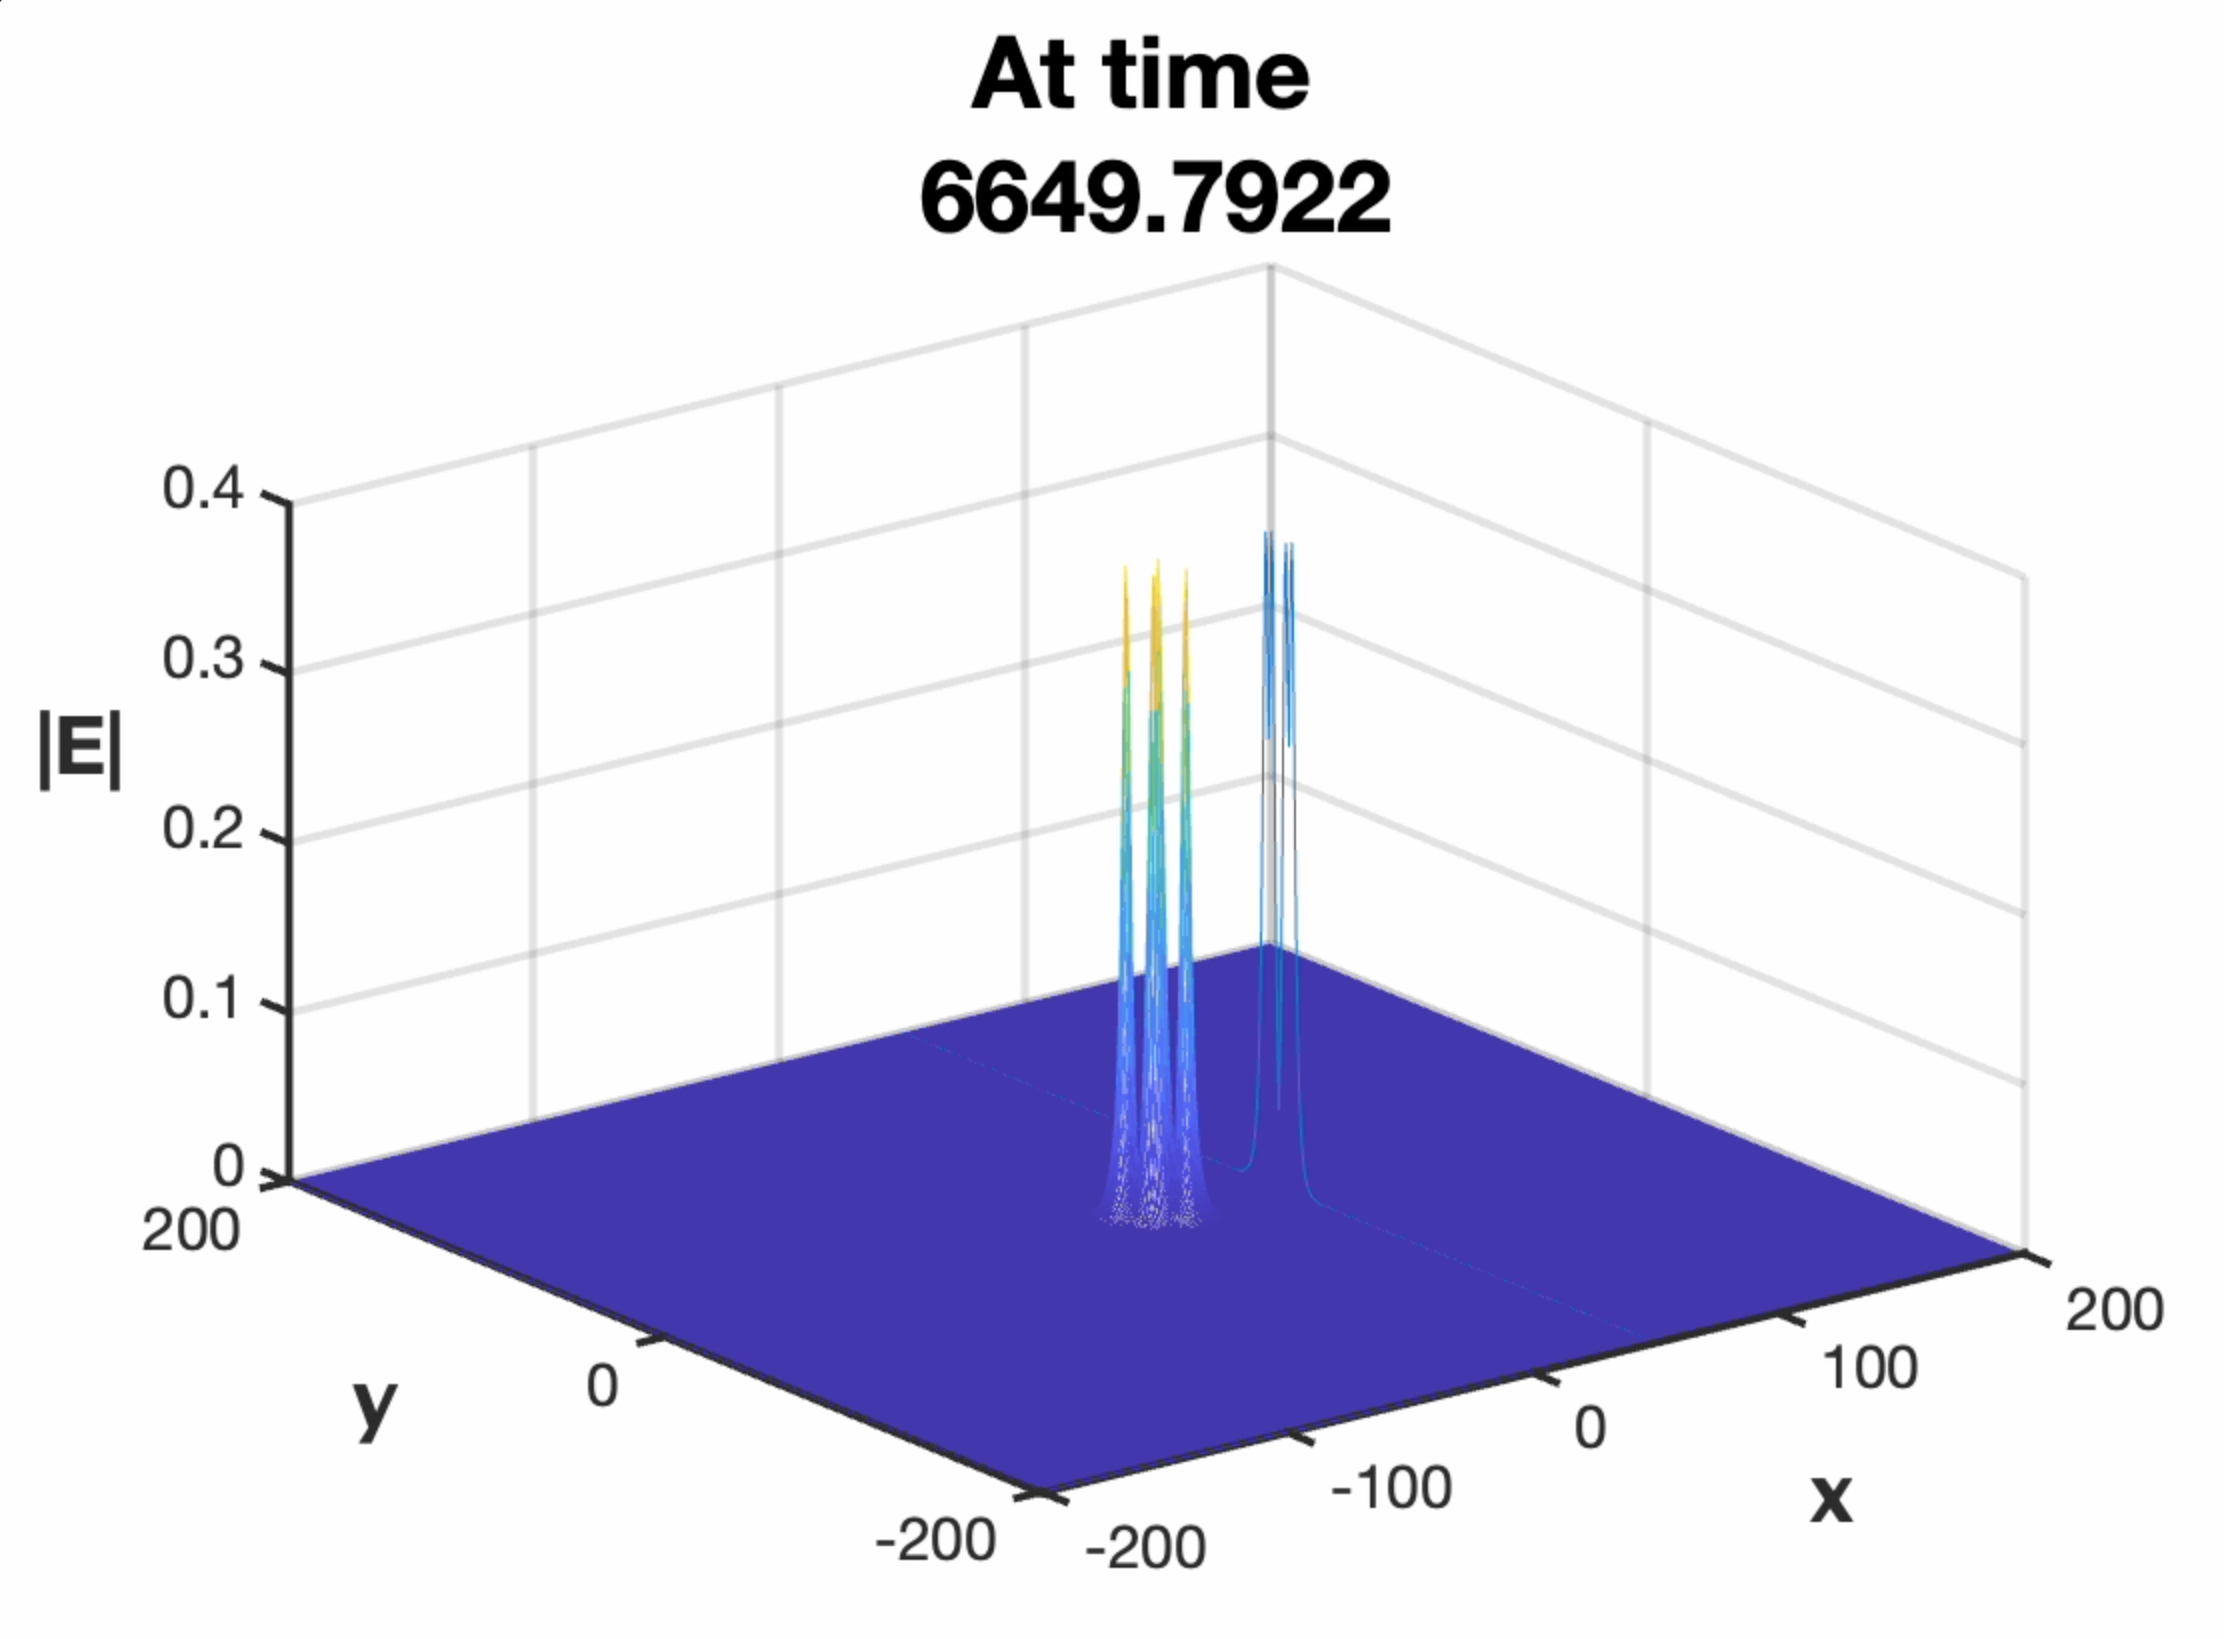
\includegraphics[scale=0.225]{TCMSG_10.png}
        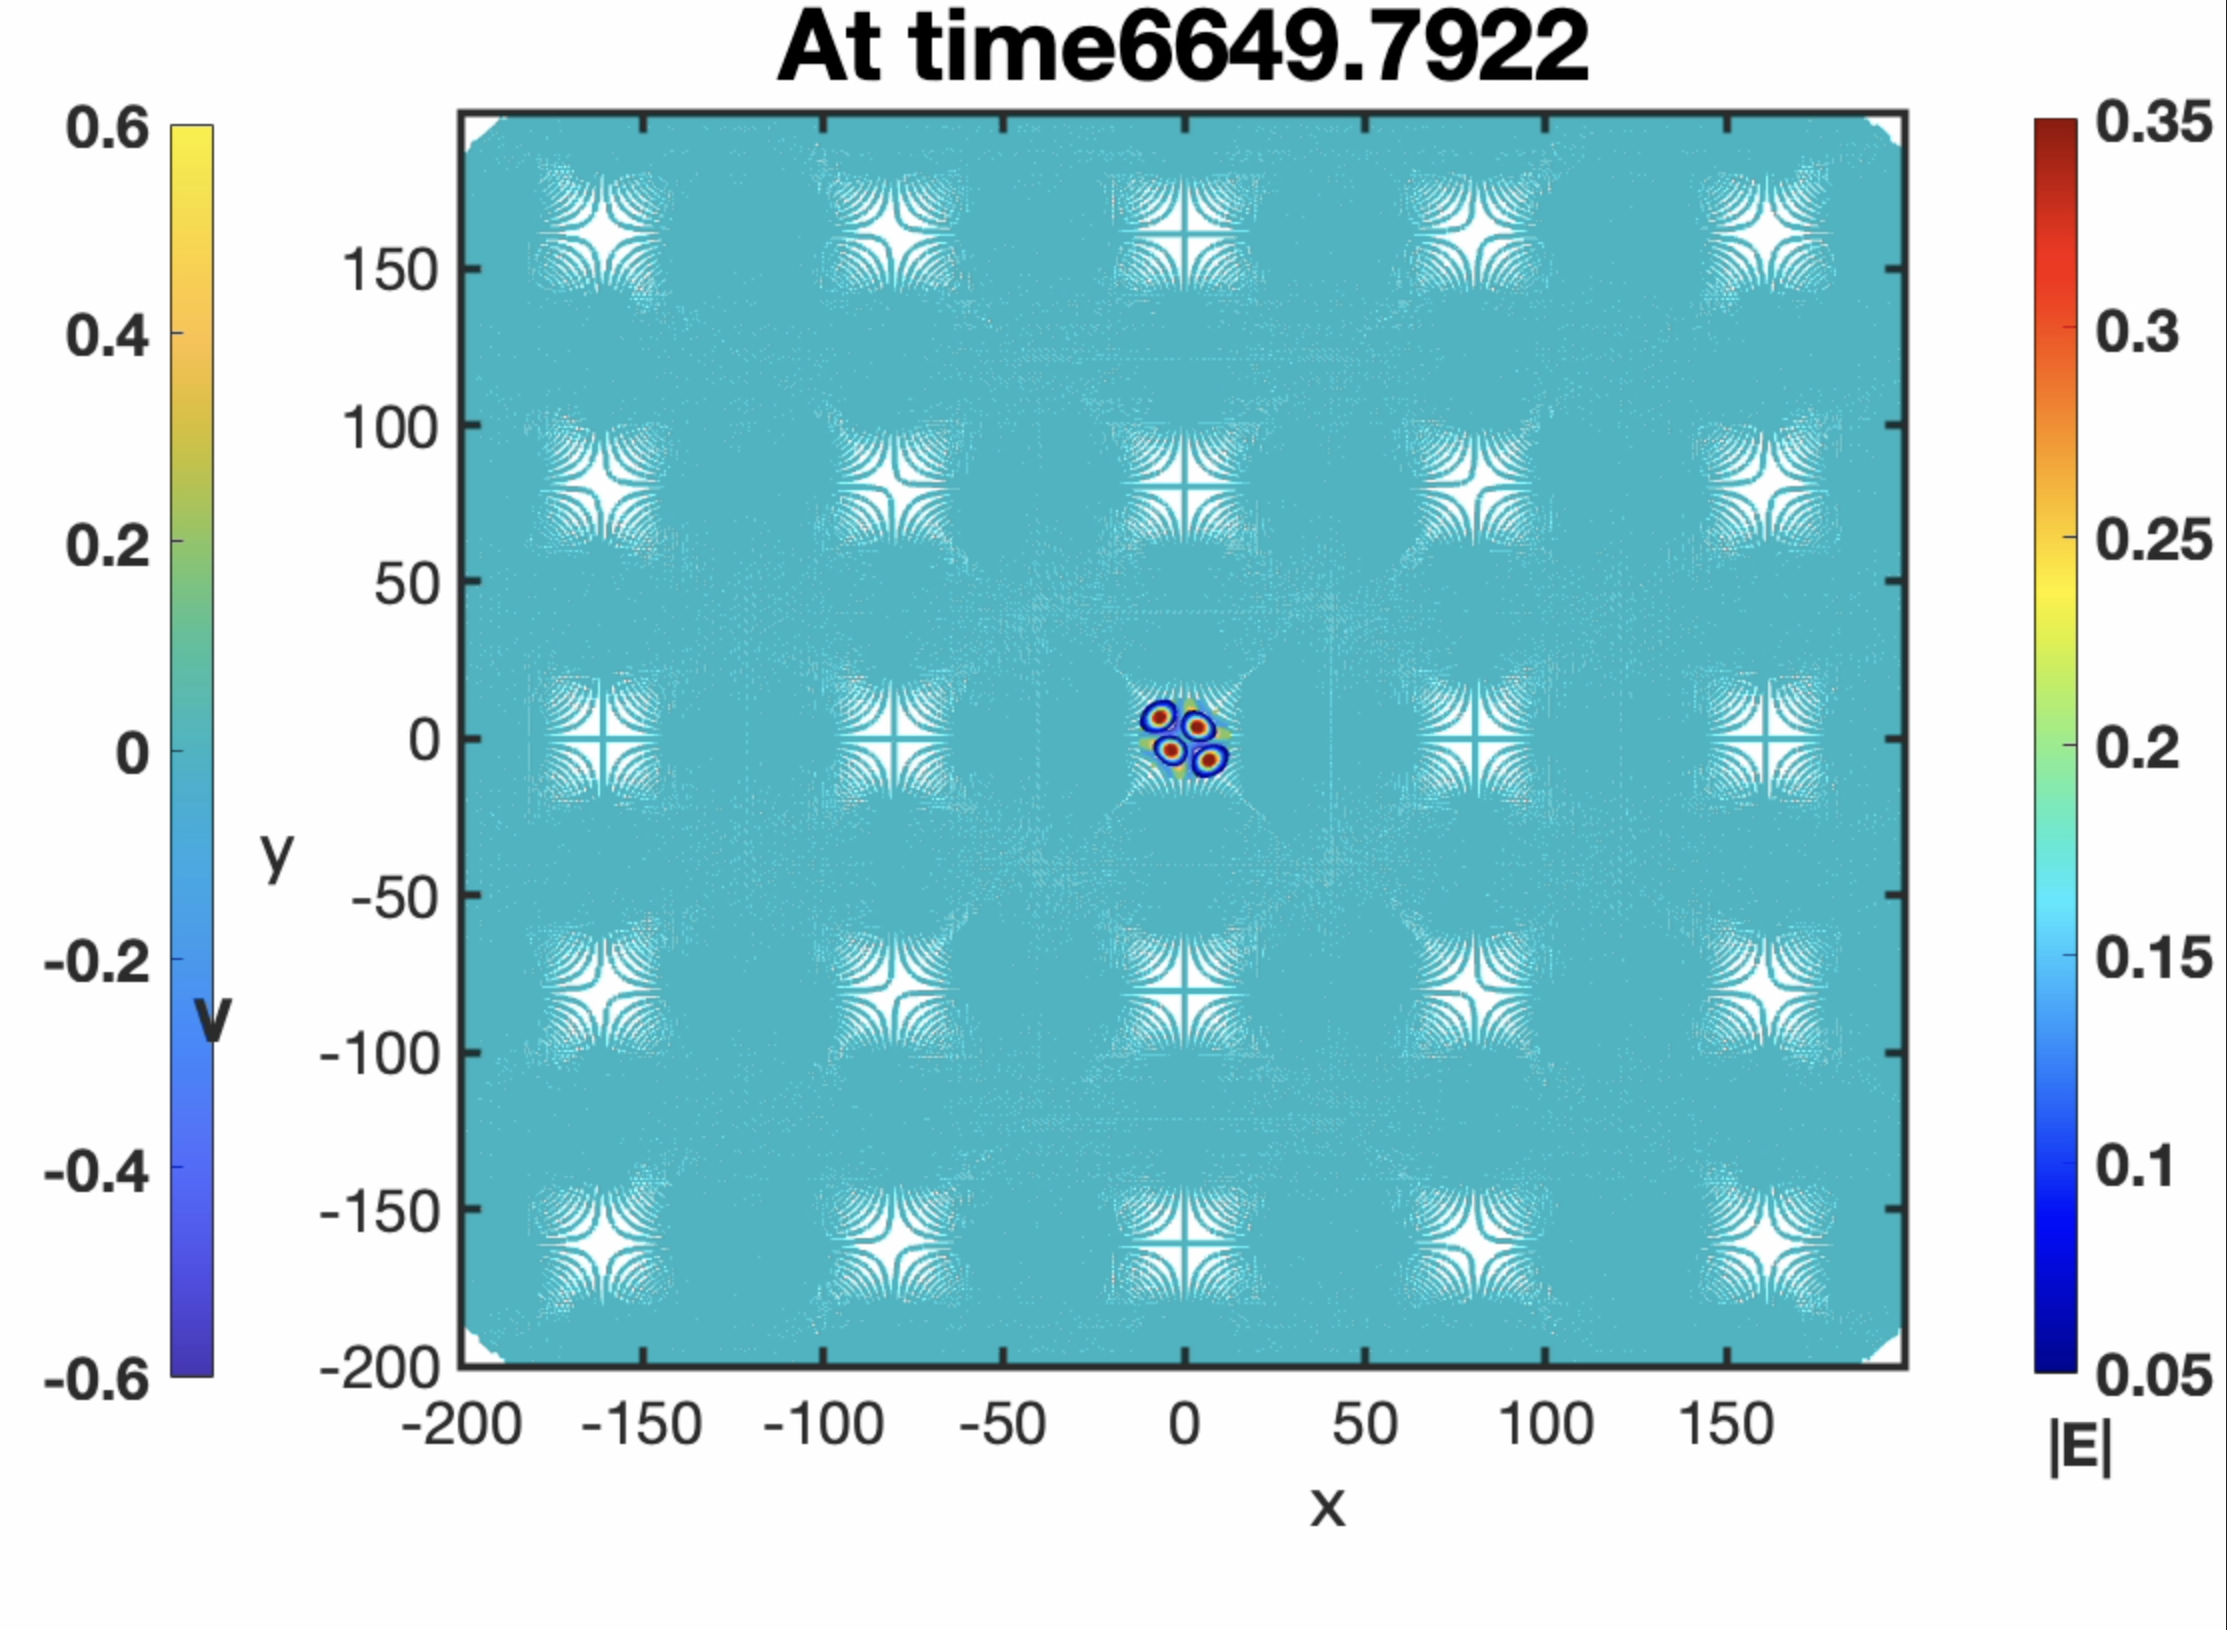
\includegraphics[scale=0.225]{TCMSG_cont_10.png}
        \caption{Soliton Trapping in TCMSG Potential}
        \label{fig:TCMSG_with_gaussian_profile}
\end{figure}

\newpage
\subsection{Sinc potential with TCMSG wave profile:}
Again we used the ring shaped Sinc potential \ref{fig:2D_Sinc_potential}, but this time with TCMSG wave profile \ref{fig:TCMSG_profile1} instead of gaussian.\
Here as well we get our solitons trapped around the central peak (\ref{fig:Sinc_with_TCMSG_profile}) of Sinc if the frequency\
of the rings and height of the potential are correctly balanced. However, an interesting discovery for this case\
was that with slight controlled imbalance, the solitons seems to oscillate towards and away from the central peak. 
\begin{figure}[H]
    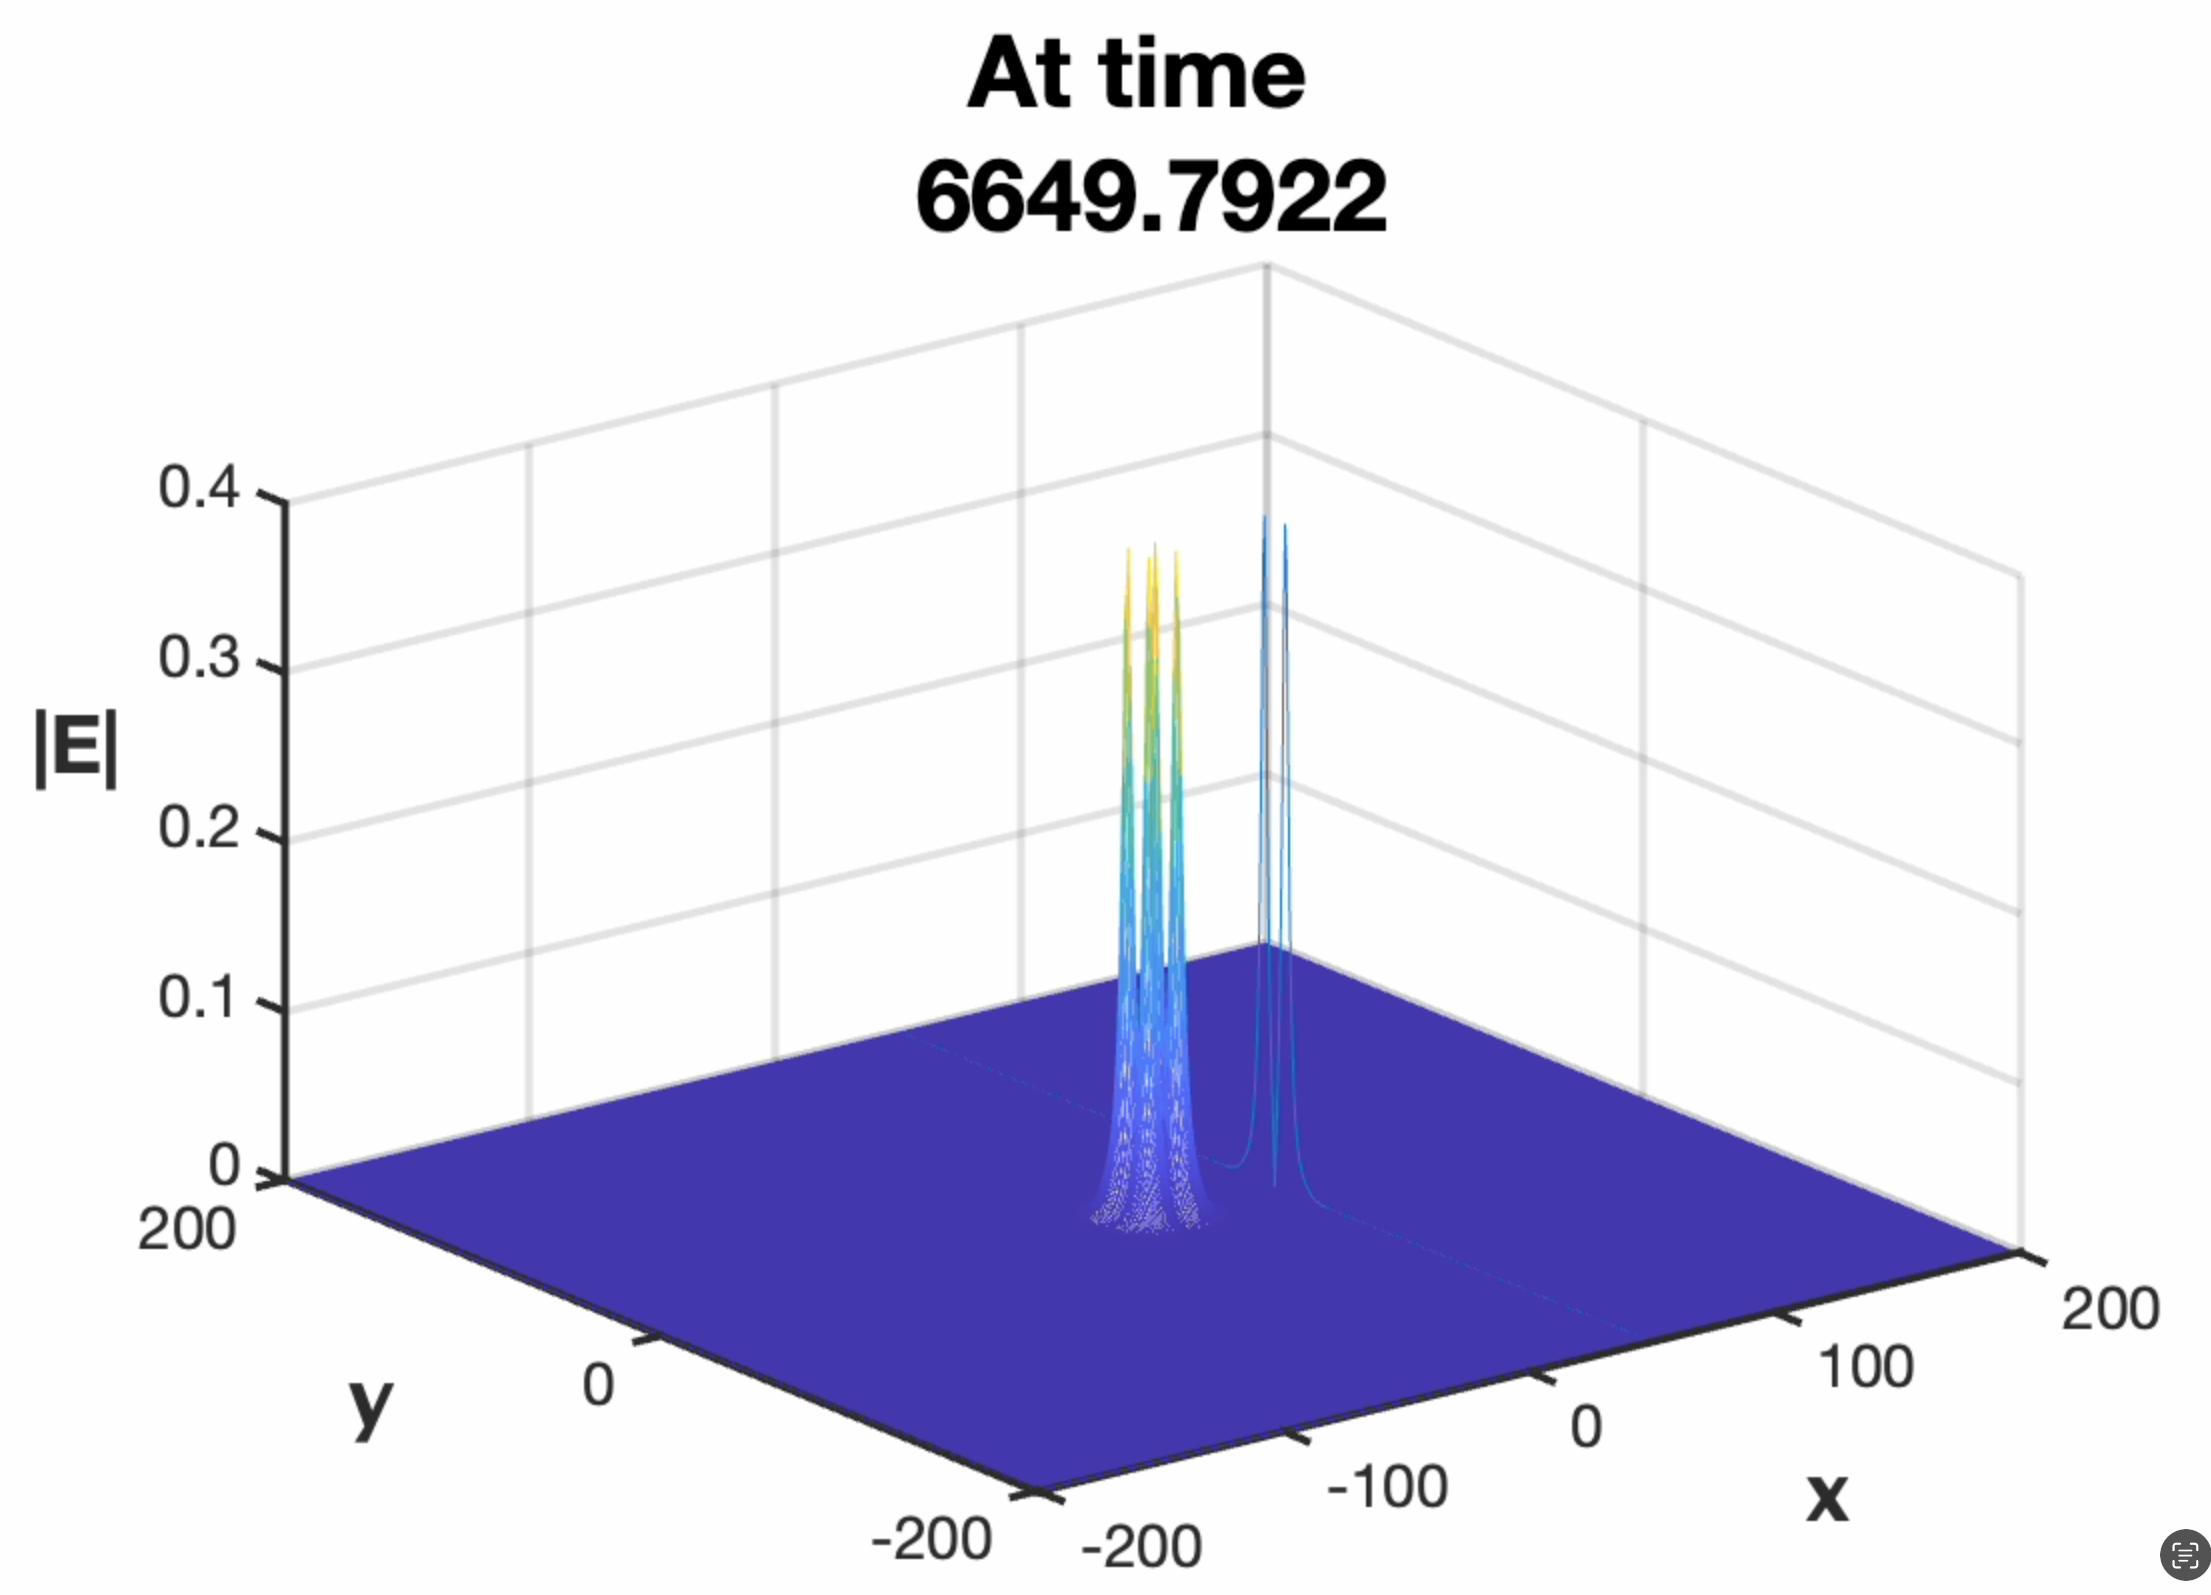
\includegraphics[scale=0.225]{Sinc_160-22.png}
    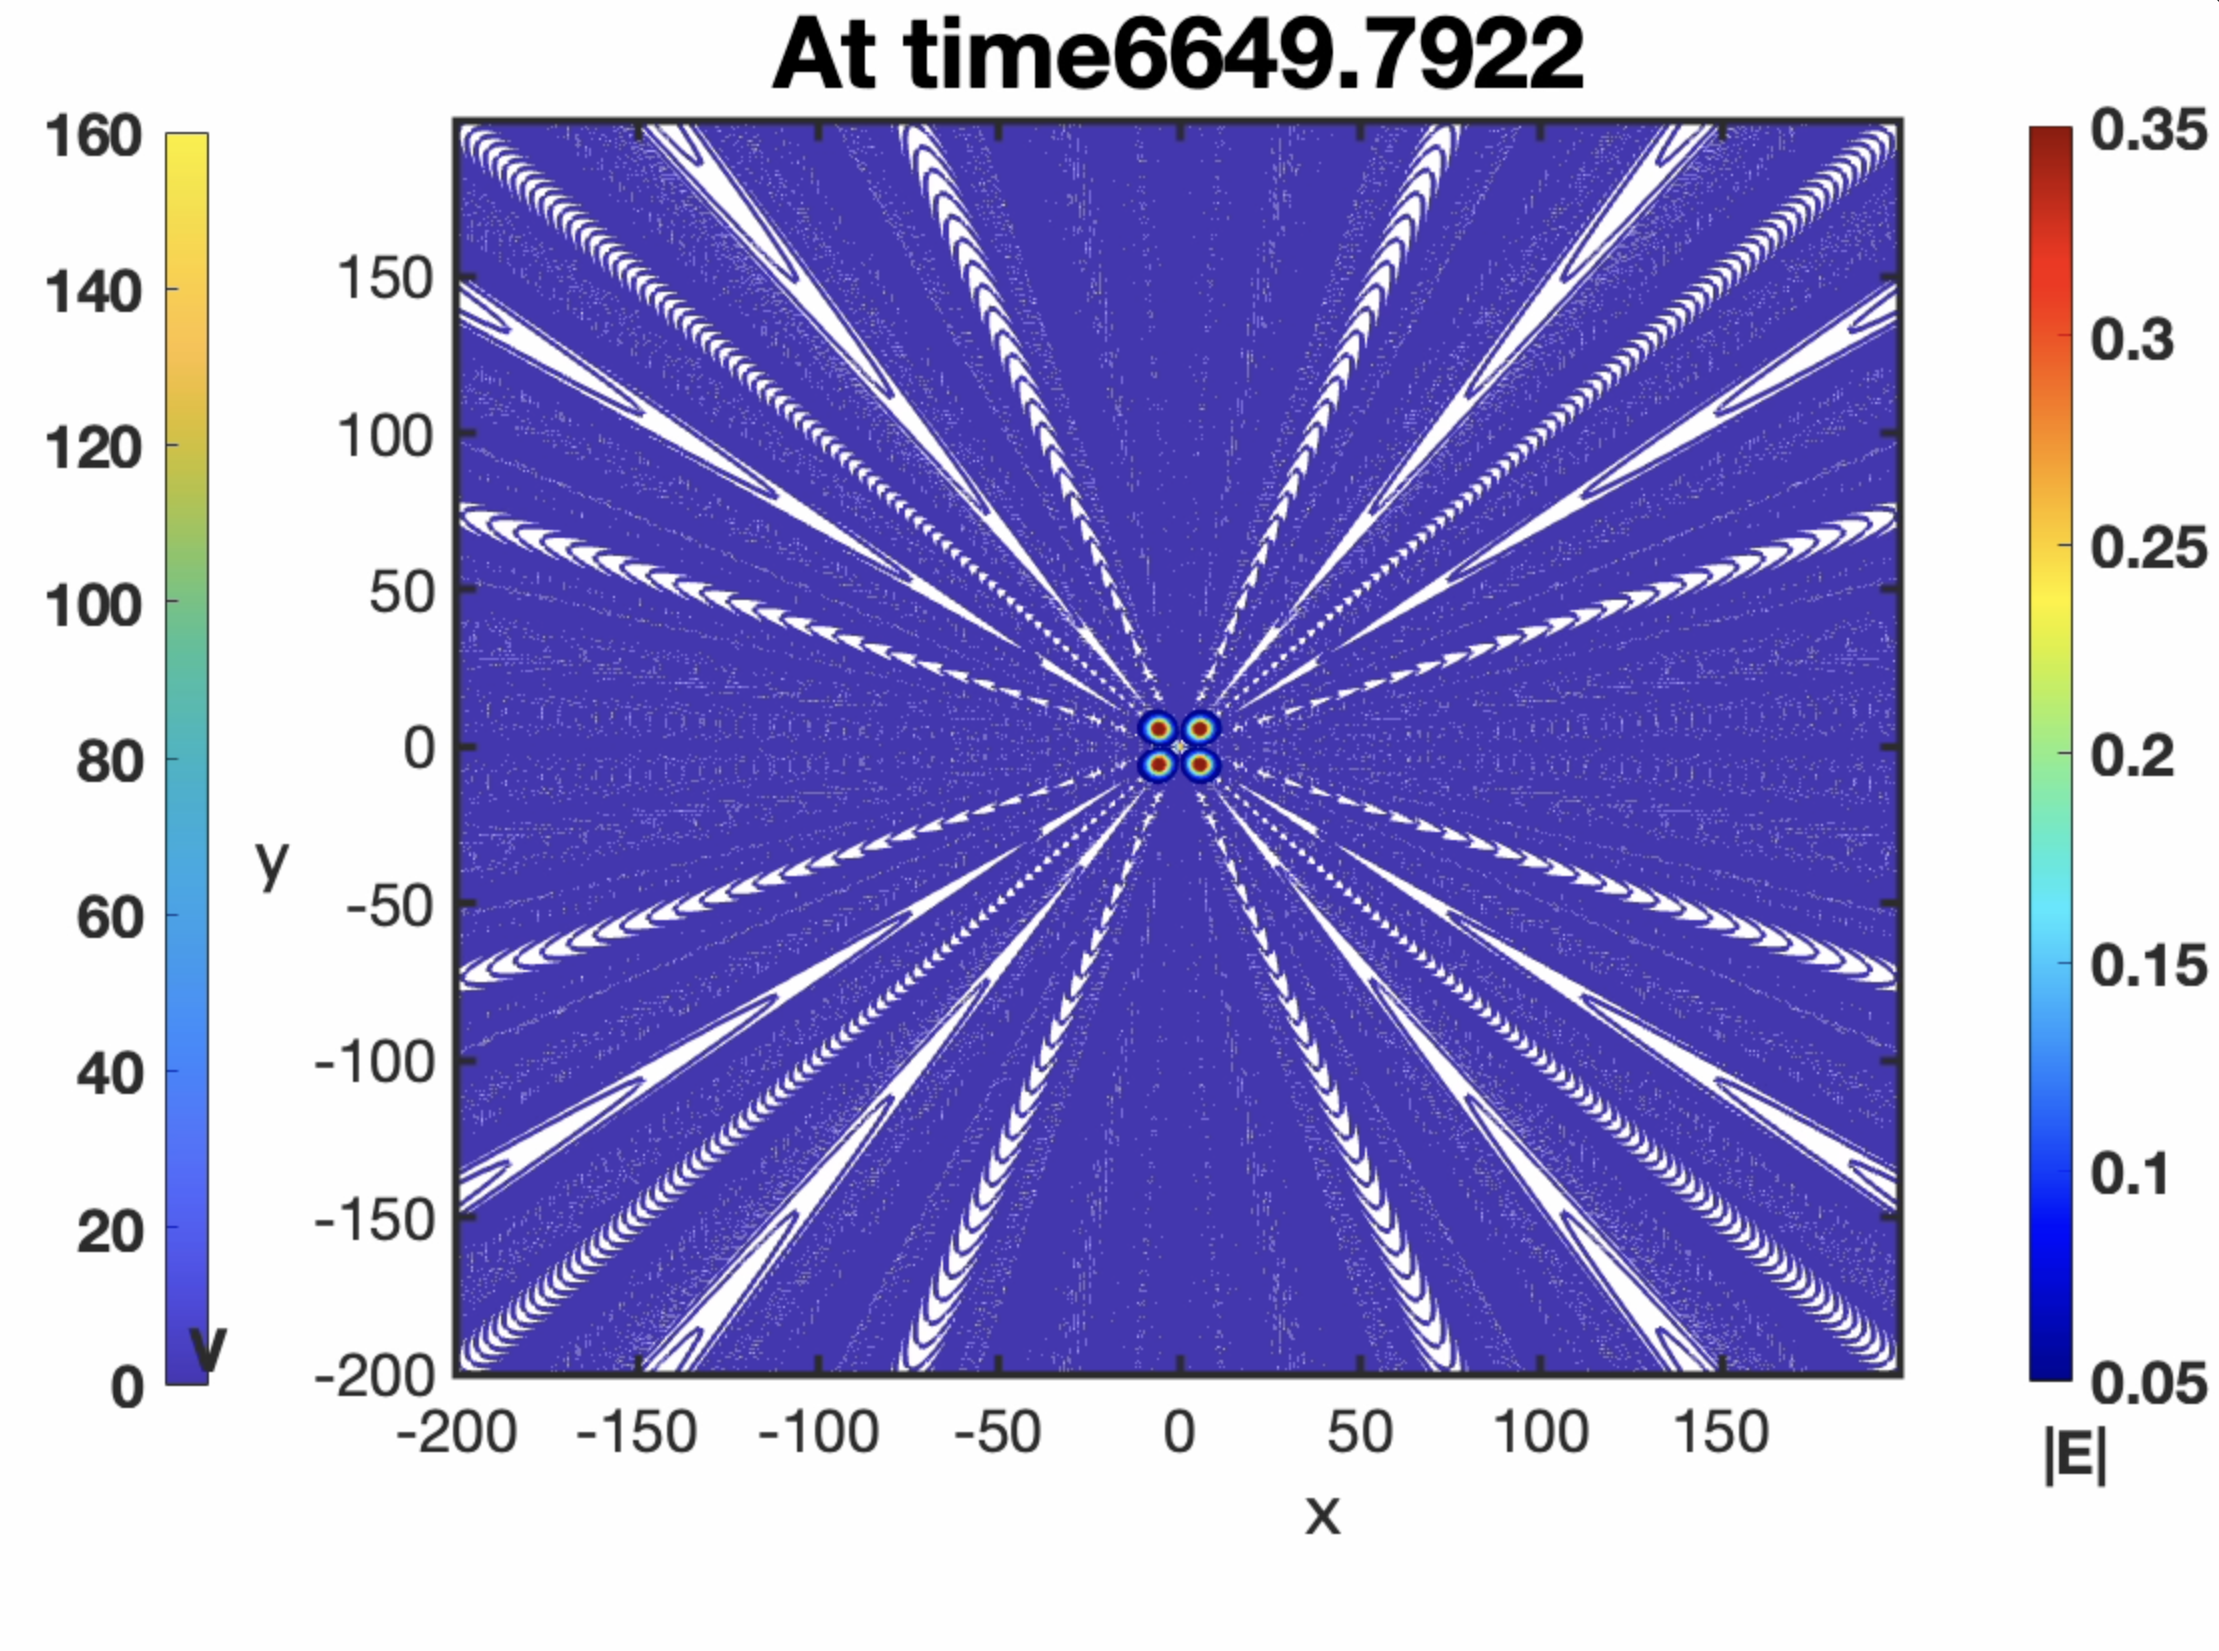
\includegraphics[scale=0.225]{Sinc_cont_160-22.png}
    \caption{Soliton Trapping in Sinc Potential with TCMSG wave profile} 
        \label{fig:Sinc_with_TCMSG_profile}
\end{figure}


\subsection{WGM like potential with Gaussian wave profile:}
Another interesting system we looked at was inspired by the famous whispering gallery phenomenon.\
In optics, whispering gallery modes (WGMs) specifically refer to the propagation of light waves along\
the curved boundary of a circular or spherical cavity. These modes are characterized by:
\begin{enumerate}
    \item \textbf{Total Internal Reflection:} Light waves undergo multiple total internal reflections along the\
    curved surface of the cavity, allowing them to propagate with minimal loss.
    \item \textbf{Resonant Frequencies:} Only certain wavelengths of light, corresponding to specific modes, satisfy\
    the condition for constructive interference after multiple reflections. This results in sharply defined resonances at particular frequencies.
\end{enumerate}

For this system we used another compound function of Bessel and gaussian functions given by (\ref{Bessel_gaussian_eqn})
\begin{equation}
    V(r) = A \exp(\frac{-r^2}{\omega}) J_n(\alpha r) \label{Bessel_gaussian_eqn}
\end{equation}
Here,  $A$  is the amplitude, $\omega$ controls the width of the Gaussian peak,\
$n $ determines the number of rings, and  $\alpha$  adjusts the spacing of the rings.

The potential looks as shown in fig (\ref{fig:bessel_gaussian_profile}).
\begin{figure}[H]
    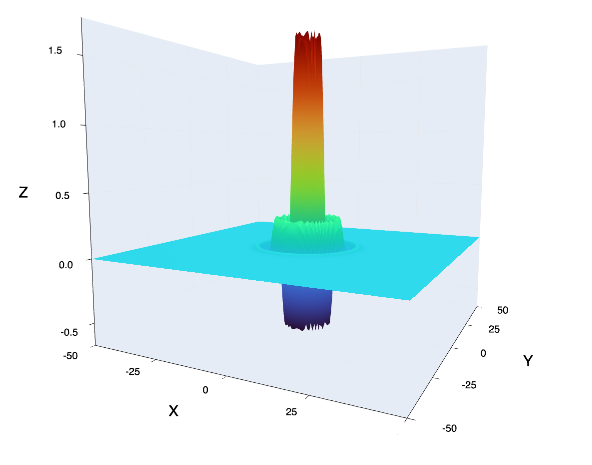
\includegraphics[scale=0.3]{bessel-gaussian-profile.png}
    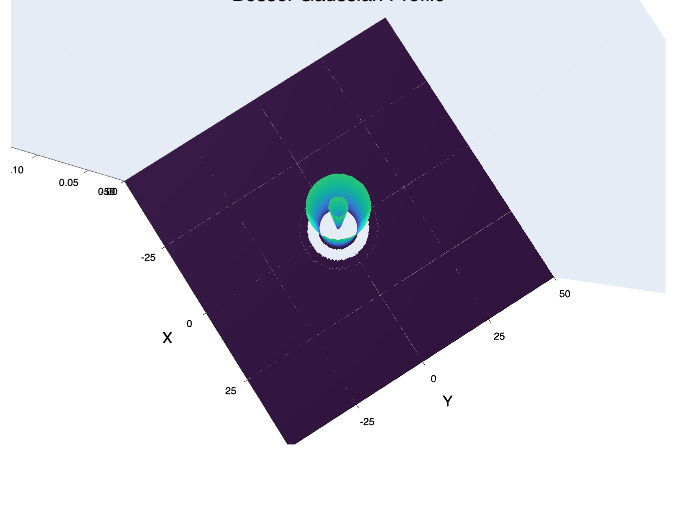
\includegraphics[scale=0.3]{bessel-gaussian-ariel.png}
    \caption{Bessel-Gaussian Profile}
    \label{fig:bessel_gaussian_profile}
\end{figure}

\begin{figure}[H]
    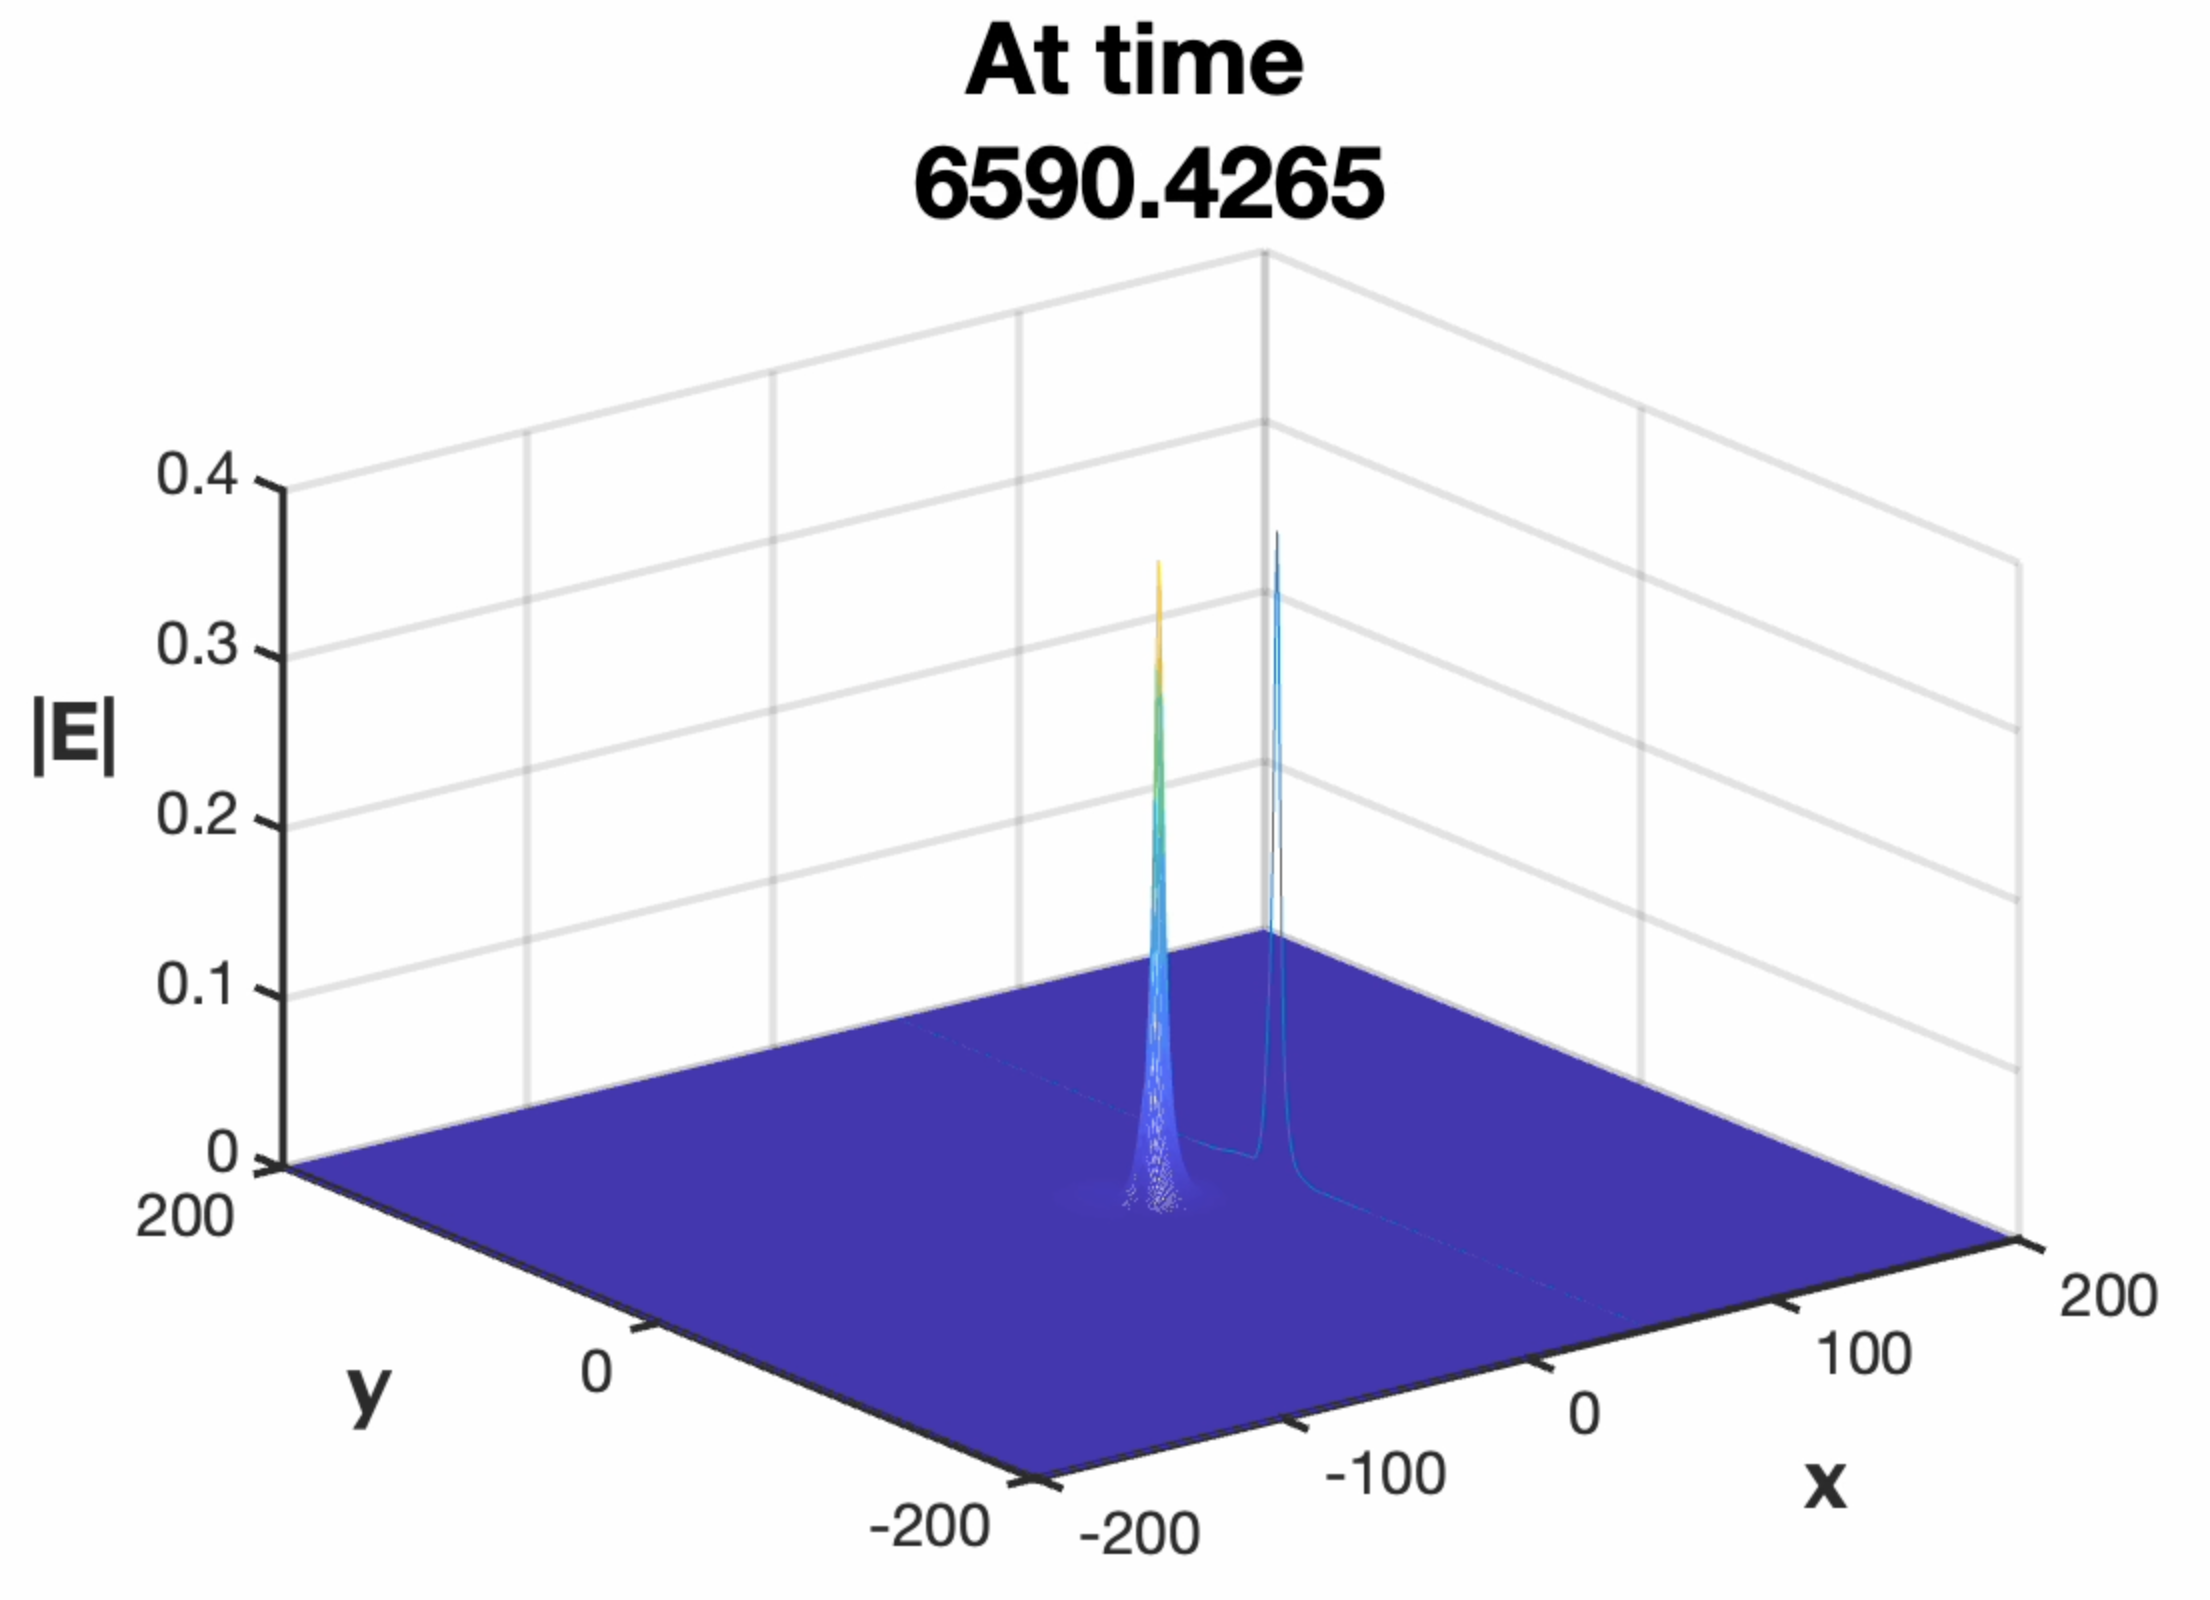
\includegraphics[scale=0.225]{3Bessel_5-1.png}
    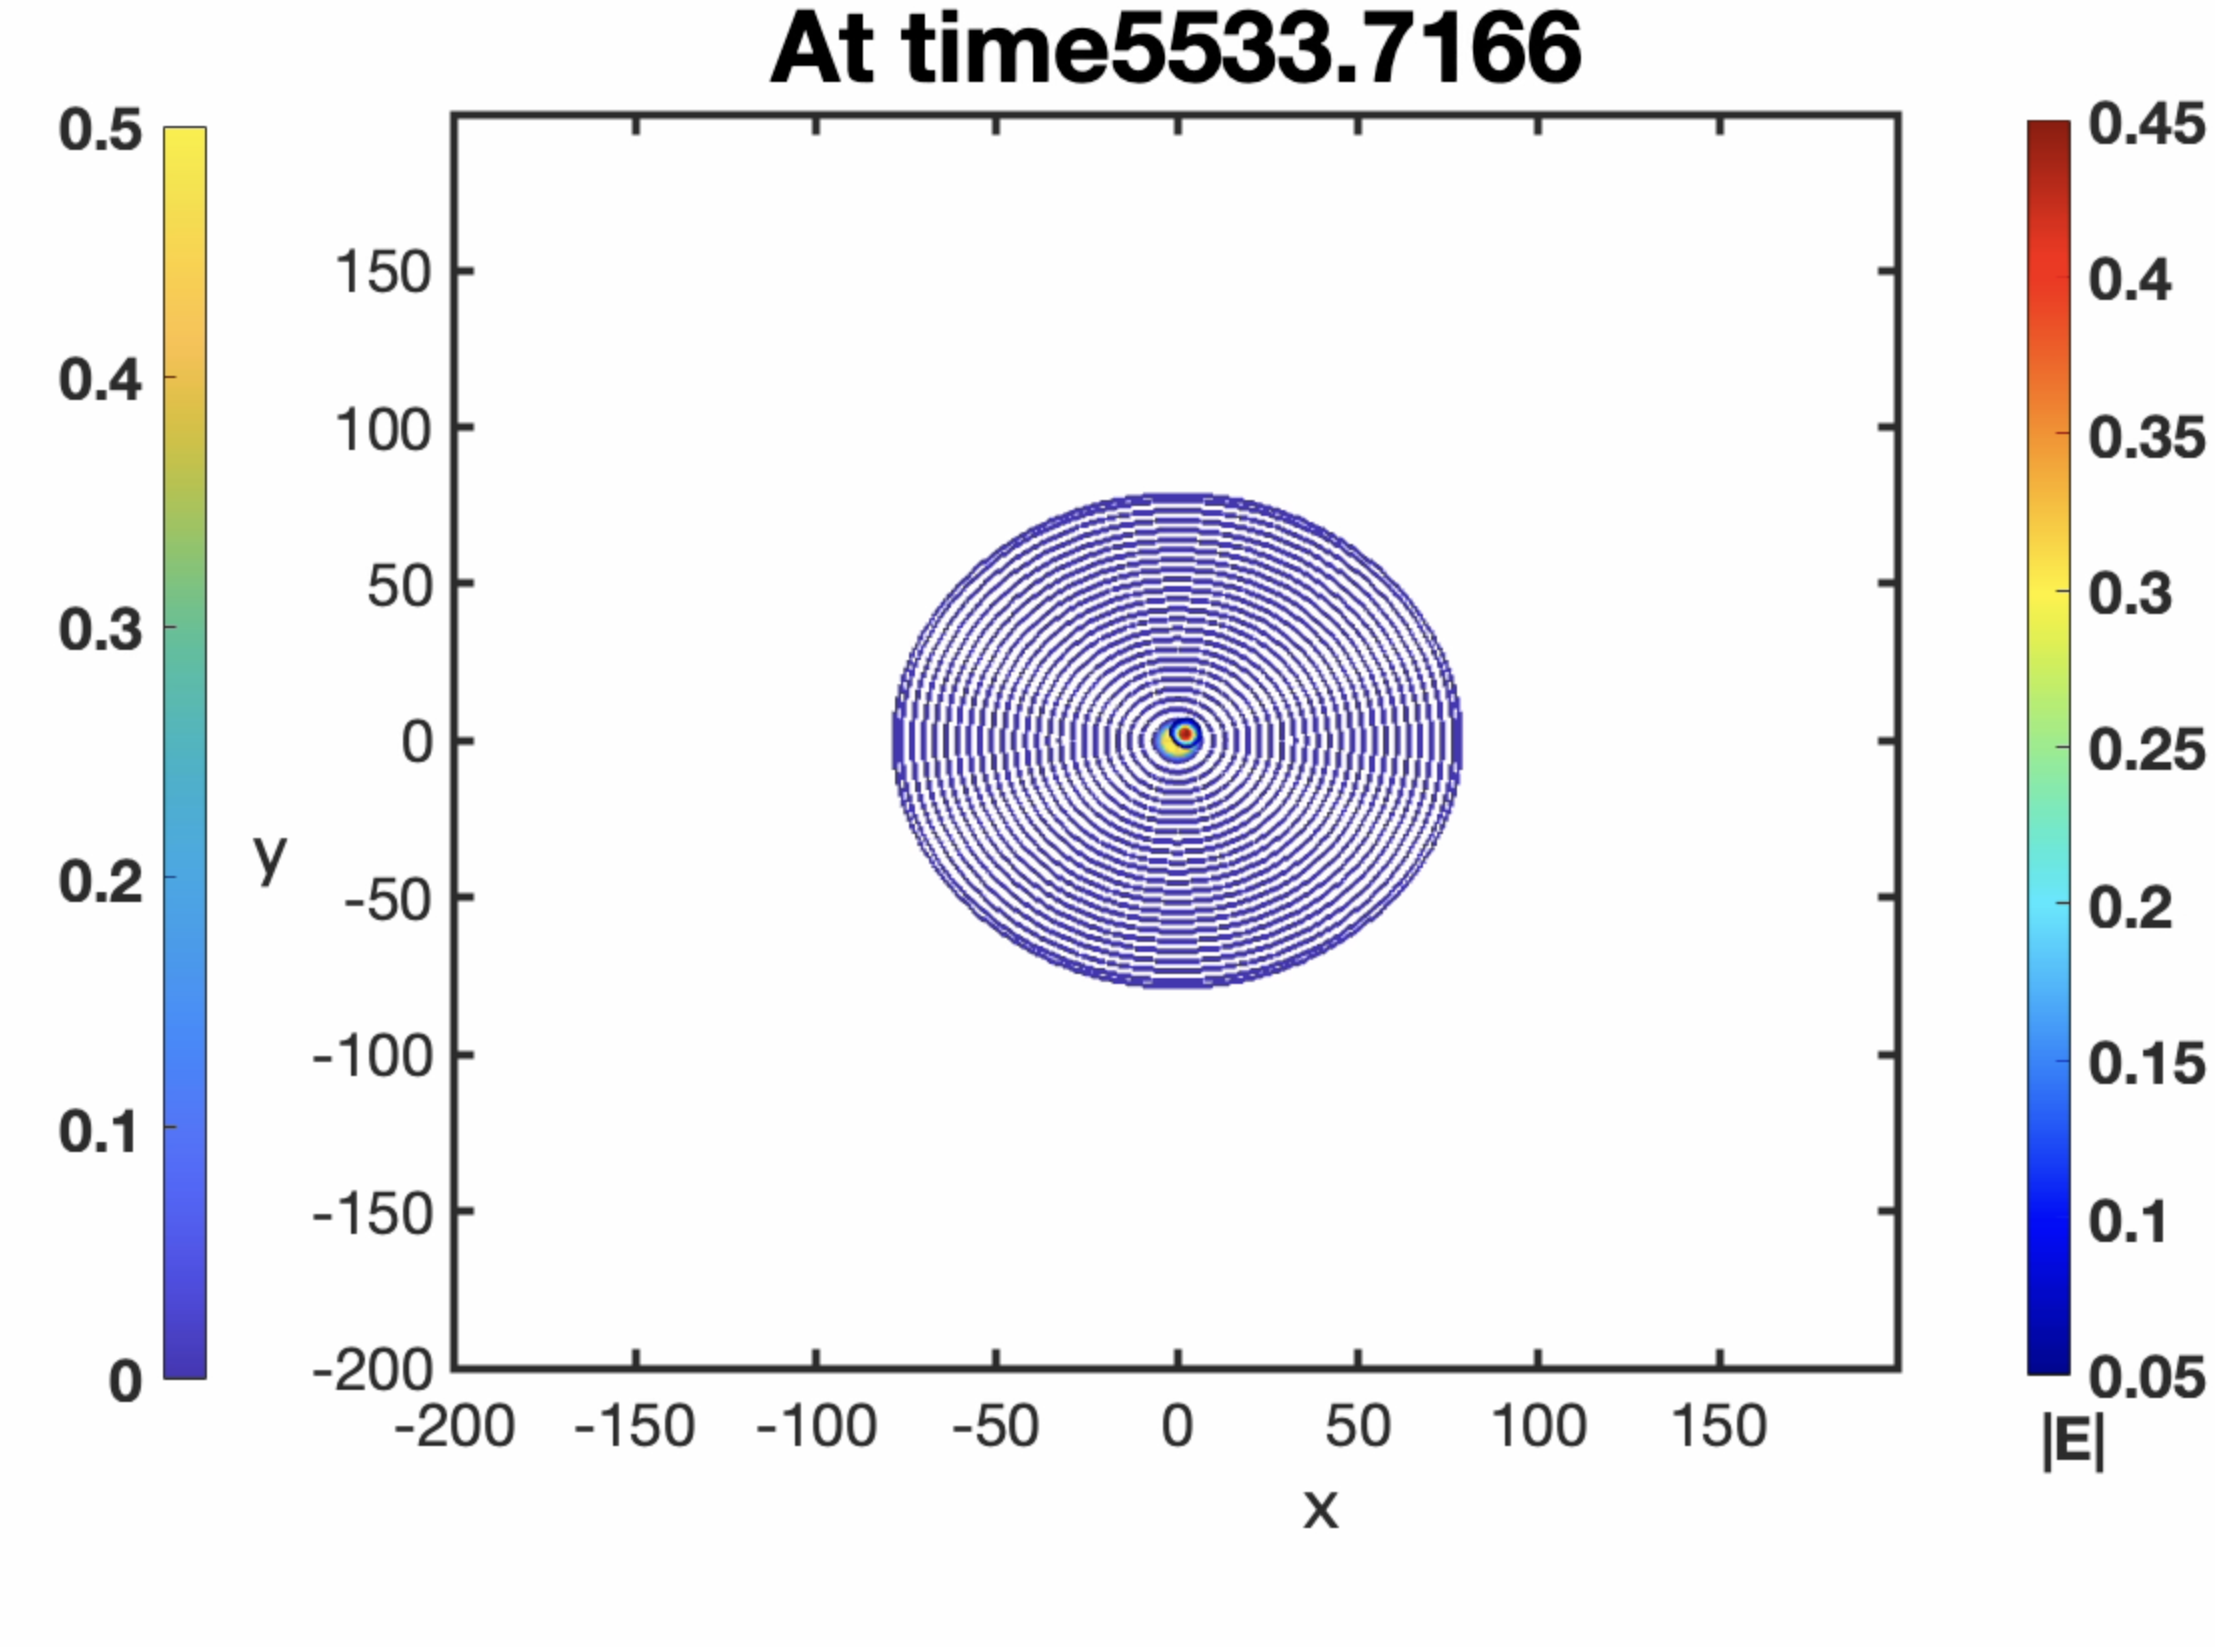
\includegraphics[scale=0.225]{3Bessel_cont_5-1.png}
    \caption{Soliton Trapping in WGM like potential with gaussian wave profile} 
        \label{fig:WGM_potential_with_gaussian_profile}
\end{figure}

This showed very interesting concentric rings that can be adjusted by varying n in (\ref{Bessel_gaussian_eqn}).
The cavity soliton formed here is trapped in the in inner most ring and keeps rotating on along the boundary.
This particular system showed the most resilience to slight changes in parameters. This might be due to extra enforcement by surrounding concentric rings.\
However due to the natural uneven shape of the bessel function, no complete stationary solitons were observed. Instead they kept moving inside the innermost ring.

\section{Stability Analysis}
For any localized structure or pattern the stability (and instability) is a big issue for application as well as for fundamental concept of the dynamics of the system. Therefore,  it is customary (as well as essential) to analyze the stability of the CS under the influence of different potentials.\\
We performed the stability analysis with respect to the significant system parameters like pumping parameter for active medium $\mu$ and feedback strength $\sigma$  for CS in the above discussed systems.\
Here we employed, largest Lypunov Exponent method to numerically analyse the stability of the above mentioned systems.\footnote[1]{The code is available on the following link: ...} The Lypunov exponent, as given by (\ref{Eqn:Lypunov Exponent}), measures the average rate of convergence or divergence\ 
of nearby trajectories, thereby acting as a description for chaotic systems \cite{kulikovEquilibriumStatesVariational2017}. They also describe how senstive the system is to the initial conditions.

\begin{equation}
    \lambda = \lim_{t\rightarrow\infty} \lim_{\delta\rightarrow 0} \frac{1}{t} \ln \frac{d(t)}{\delta} \label{Eqn:Lypunov Exponent}
\end{equation}
Where d is the separation between the trajectories at a given time t, and $\delta$ is the initial purturbation.


The steady state solution of the system are found by directly solving the differential equation for steady state condition. 
The Maximal Lyapunov Exponent is numerically calculated as follows:

\begin{enumerate}
    \item First find the steady state solution by directly solving the differential equation.
    \item Create a perturbed state $E_{perturbed} = E + \delta$, where $\delta$ is a small perturbation
    \item Evolve both E and $E_{perturbed}$ 
    \item Calculate the new seperation $d = || E_{new} - E_{new perturbed}||$
    \item Compute the local Lypunov exponent : $ \lambda_{local} = \ln (d/\sigma) /\Delta t $
    \item Repeat the process many times (1000 iterations are taken for our code)
    \item Calculate the final Lypunov exponent by averaging all the local exponents $\lambda = (1/N) \sum \lambda_{local}$
\end{enumerate}

The Largest or Maximal Lyapunov Exponent, gives us a good idea about the stability of the system. Negative or smaller values 
correspond to the stable system, while positive or larger value corresponds to unstability.


The following figures Fig: \ref{fig:Stability analysis for gaussian profiles} \& Fig: \ref{fig:Stability analysis for TCMSG profiles} 
shows the stability analysis of systems with initial profile to be gaussian and TCMSG respectively.
\begin{enumerate}
    \item The first figure is a 3D landscape of Lyapunov Exponent on the z axis as the $\mu$ and $\sigma$ are changing.
    \item The second figure shows how the exponent is changing with respect to $\sigma$ while $\mu$ is constant at 0.5.
    \item The third figure show similar to previous, how the exponent is changing with respect to $\mu$ while $\sigma$ is kept constant at 0.5.
    \item The fourth is the contour plot showing the region for which the system shows stability.
    \item The fifth figure is the heatmap of Lyapunov exponent for the values of $\mu$ and $\sigma$.
    \item The figures sixth to ninth, shows the phase plot of the system for different values of $\mu$ and $\sigma$.
\end{enumerate}


\begin{figure}[H]
        \centering
        \begin{subfigure}[b]{0.31\textwidth}
            \centering
            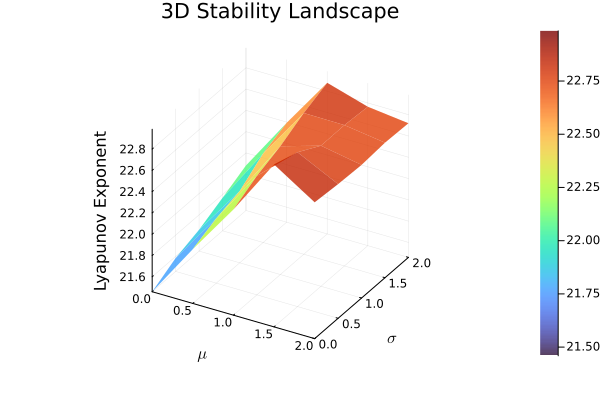
\includegraphics[scale=0.3]{gaussian_stab/Bessel-Gaussian _lyapunov_3d_surface.png}
            \label{fig:gaussian_stability1}
            \caption{}
        \end{subfigure}
        % \hfill
        \begin{subfigure}[b]{0.31\textwidth}
            \centering
            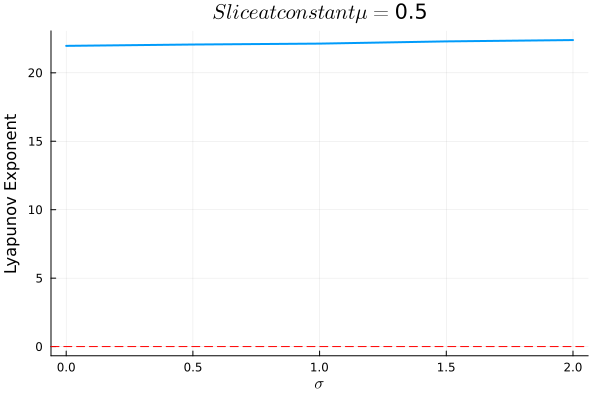
\includegraphics[scale=0.3]{gaussian_stab/Bessel-Gaussian _mu_slice_plot.png}
            \label{fig:gaussian_stability2}
            \caption{}
        \end{subfigure}
        % \hfill
        \begin{subfigure}[b]{0.31\textwidth}
            \centering
            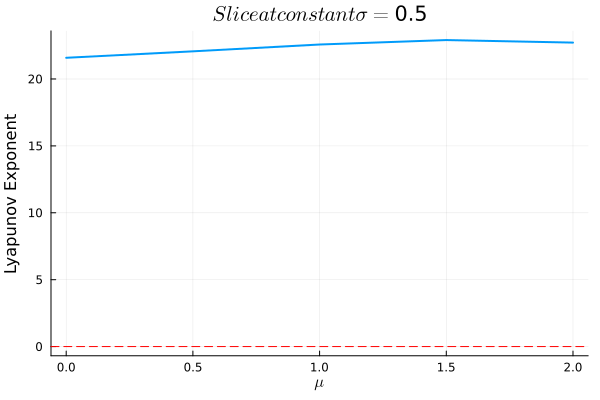
\includegraphics[scale=0.3]{gaussian_stab/Bessel-Gaussian _sigma_slice_plot.png}
            \label{fig:gaussian_stability3}
            \caption{}
        \end{subfigure}
        
        \vspace{0.2cm} % add vertical space
        
        \begin{subfigure}[b]{0.31\textwidth}
            \centering
            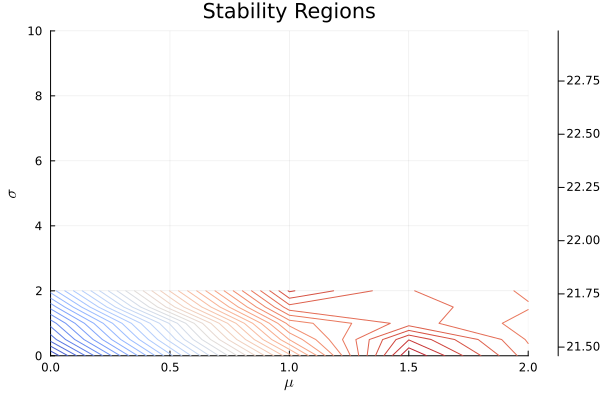
\includegraphics[scale=0.3]{gaussian_stab/Bessel-Gaussian _stability_regions_contour.png}
            \label{fig:gaussian_stability4}
            \caption{}
        \end{subfigure}
        % \hfill
        \begin{subfigure}[b]{0.31\textwidth}
            \centering
            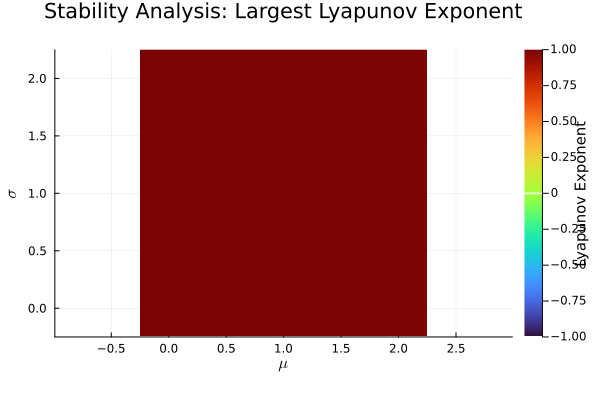
\includegraphics[scale=0.3]{gaussian_stab/Bessel-Gaussian_lyapunov_heatmap.png}
            \label{fig:gaussian_stability5}
            \caption{}
        \end{subfigure}
        % \hfill
        \begin{subfigure}[b]{0.31\textwidth}
            \centering
            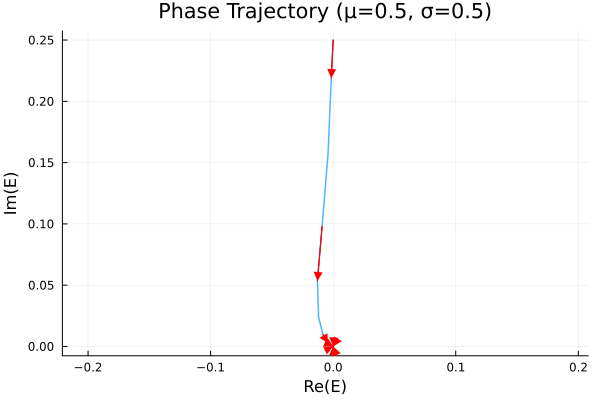
\includegraphics[scale=0.3]{gaussian_stab/Bessel-Gaussian_phase_trajectory_1.png}
            \label{fig:gaussian_stability6}
            \caption{}
        \end{subfigure}
        
        \vspace{0.2cm} % add vertical space
        
        \begin{subfigure}[b]{0.31\textwidth}
            \centering
            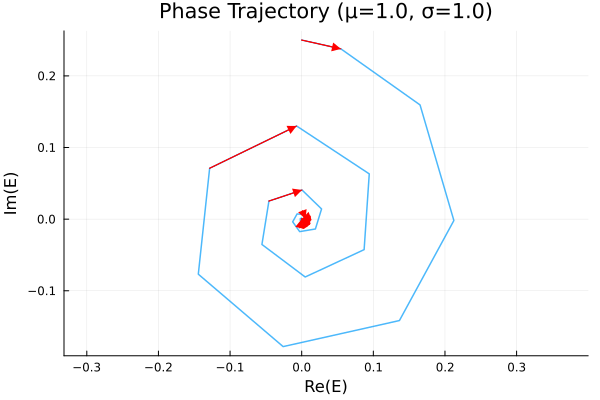
\includegraphics[scale=0.3]{gaussian_stab/Bessel-Gaussian_phase_trajectory_2.png}
            \label{fig:gaussian_stability7}
            \caption{}
        \end{subfigure}
        % \hfill
        \begin{subfigure}[b]{0.31\textwidth}
            \centering
            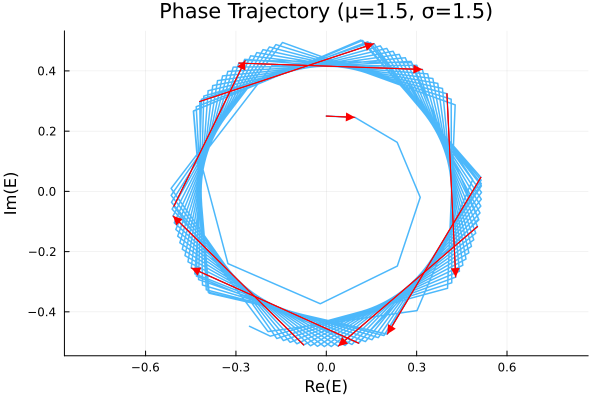
\includegraphics[scale=0.3]{gaussian_stab/Bessel-Gaussian_phase_trajectory_3.png}
            \label{fig:gaussian_stability8}
            \caption{}
        \end{subfigure}
        % \hfill
        \begin{subfigure}[b]{0.31\textwidth}
            \centering
            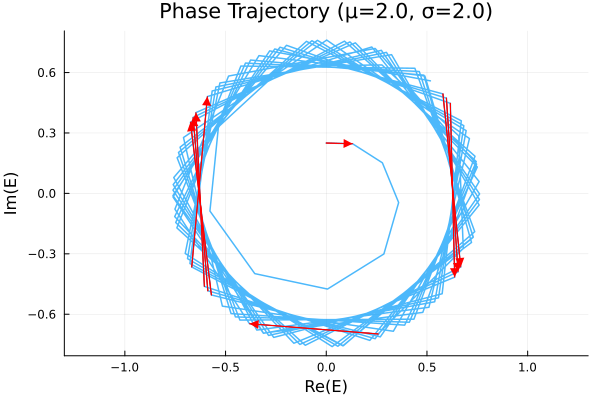
\includegraphics[scale=0.3]{gaussian_stab/Bessel-Gaussian_phase_trajectory_4.png}
            \label{fig:gaussian_stability9}
            \caption{}
        \end{subfigure}
        
        \caption{Stability Analysis for the Gaussian input profiles}
        \label{fig:Stability analysis for gaussian profiles}
\end{figure}

\begin{figure}[H]
    \centering
    \begin{subfigure}[b]{0.31\textwidth}
        \centering
        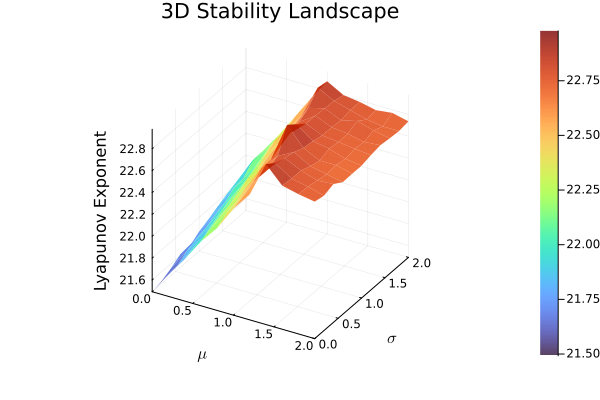
\includegraphics[scale=0.3]{tcmsg_stab/Sinc_tcmsg_profile_lyapunov_3d_surface.png}
        \label{fig:tcmsg_stability1}
        \caption{}
    \end{subfigure}
    % \hfill
    \begin{subfigure}[b]{0.31\textwidth}
        \centering
        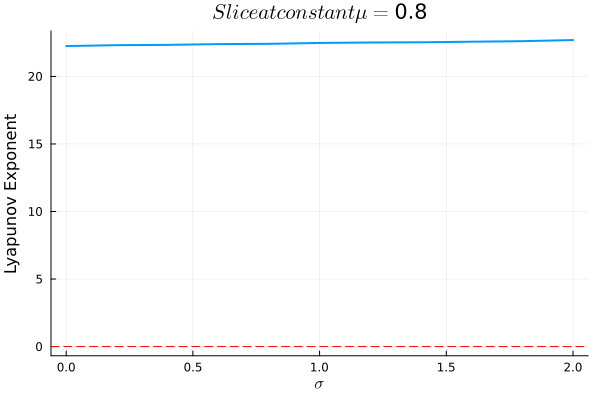
\includegraphics[scale=0.3]{tcmsg_stab/Sinc_tcmsg_profile_mu_slice_plot.png}
        \label{fig:tcmsg_stability2}
        \caption{}
    \end{subfigure}
    % \hfill
    \begin{subfigure}[b]{0.31\textwidth}
        \centering
        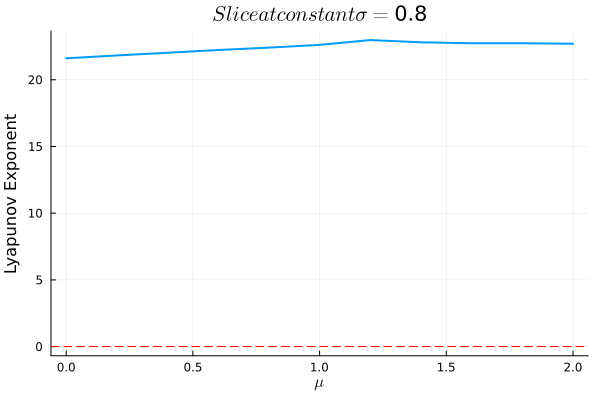
\includegraphics[scale=0.3]{tcmsg_stab/Sinc_tcmsg_profile_sigma_slice_plot.png}
        \label{fig:tcmsg_stability3}
        \caption{}
    \end{subfigure}
    
    \vspace{0.2cm} % add vertical space
    
    \begin{subfigure}[b]{0.31\textwidth}
        \centering
        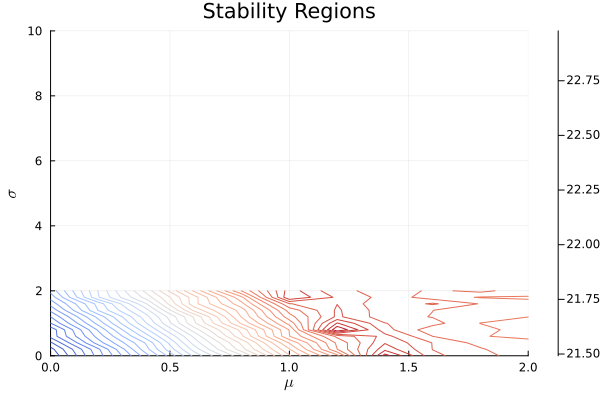
\includegraphics[scale=0.3]{tcmsg_stab/Sinc_tcmsg_profile_stability_regions_contour.png}
        \label{fig:tcmsg_stability4}
        \caption{}
    \end{subfigure}
    % \hfill
    \begin{subfigure}[b]{0.31\textwidth}
        \centering
        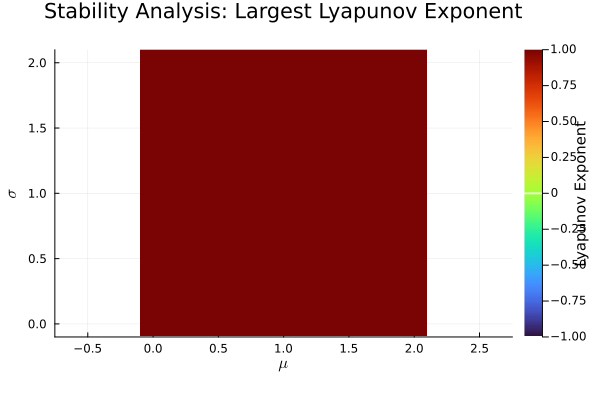
\includegraphics[scale=0.3]{tcmsg_stab/Sinc_tcmsg_profile_lyapunov_heatmap.png}
        \label{fig:tcmsg_stability5}
        \caption{}
    \end{subfigure}
    % \hfill
    \begin{subfigure}[b]{0.31\textwidth}
        \centering
        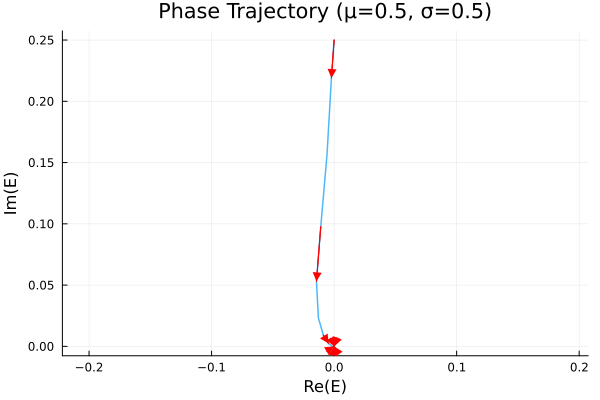
\includegraphics[scale=0.3]{tcmsg_stab/Sinc_tcmsg_profile_phase_trajectory_1.png}
        \label{fig:tcmsg_stability6}
        \caption{}
    \end{subfigure}
    
    \vspace{0.2cm} % add vertical space
    
    \begin{subfigure}[b]{0.31\textwidth}
        \centering
        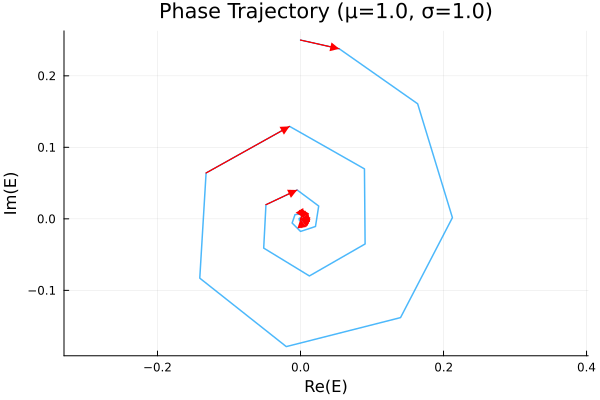
\includegraphics[scale=0.3]{tcmsg_stab/Sinc_tcmsg_profile_phase_trajectory_2.png}
        \label{fig:tcmsg_stability7}
        \caption{}
    \end{subfigure}
    % \hfill
    \begin{subfigure}[b]{0.31\textwidth}
        \centering
        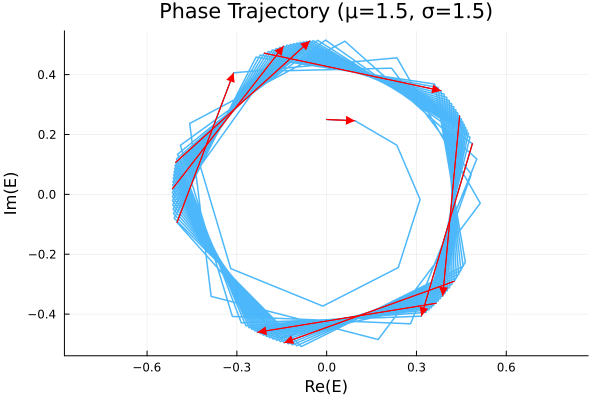
\includegraphics[scale=0.3]{tcmsg_stab/Sinc_tcmsg_profile_phase_trajectory_3.png}
        \label{fig:tcmsg_stability8}
        \caption{}
    \end{subfigure}
    % \hfill
    \begin{subfigure}[b]{0.31\textwidth}
        \centering
        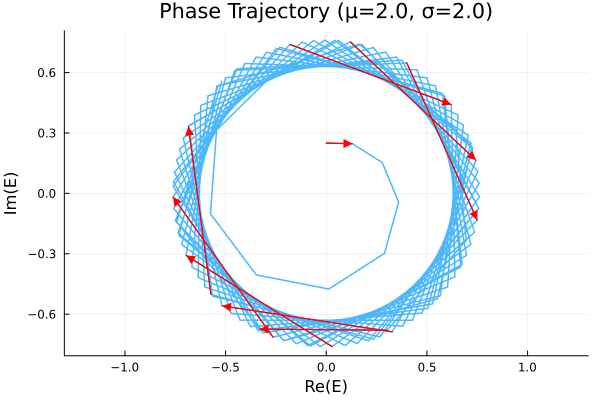
\includegraphics[scale=0.3]{tcmsg_stab/Sinc_tcmsg_profile_phase_trajectory_4.png}
        \label{fig:tcmsg_stability9}
        \caption{}
    \end{subfigure}
    
    \caption{Stability Analysis for the TCMSG input profiles}
    \label{fig:Stability analysis for TCMSG profiles}
\end{figure}


\paragraph{Results:}
The stability region for all the above system did not show any significant variation. We can see from the plots above, the system where TCMSG was the input profile (\ref{fig:Stability analysis for TCMSG profiles})\
the region of stability is slightly more for bigger values of $\mu$ than for all the other systems that had gaussian input profile (\ref{fig:Stability analysis for gaussian profiles}) stopped at $\mu=1$. While the upper value of $\sigma$ for \
which stability can be seen, is the same in both the cases. Nonetheless, the overall nature of dynamics seems to be consistent. Looking at the phase plots we see that around \
the values of $\mu =1$ and $\sigma=1$ to be equal we get a stable system, and above that the system becomes unstable and exhibits Hopf bifurcation typical of CGLE. 


